\documentclass[a4paper,10pt,twoside]{report}

\usepackage[margin=1in]{geometry}
\usepackage{amsmath}
\usepackage{titling}
\usepackage{fontspec}
\usepackage{listings}
\usepackage{hyperref}
\usepackage{graphicx}

\usepackage[dvipsnames]{xcolor}

\lstdefinelanguage{Java}{
	keywords=[1]{
		fields, schemaData, dataframe, latMin, latMax, longMin, longMax, rightOuter, leftOuter, lat1, lon1, lat2, lon2, deltaLat, deltaLon, c, d, a, radius, distance, time, tokenizer, remover, assembler, linreg, rfr, trainsetsplit, traintestsplit, indexer, minmax, pipelinerfr, paramgridrfr, pipelinelinreg, trainedlinreg, model, cvmrfr, evaluator, calc, log, metrictype, metrictypes, svc, pca, paramgridsvm, cvsvm, predictionssvm, metrics, predictionsLogReg, predictions, train, test, trainsetsplit, traintestsplit, datasets, createsubsample, pipelinesvm, glr, paramgridglr, gbt, paramgridgbt, pipelineglr, pipelinegbt, predictionsrfr, cvrfr, trainvalidationsplitglr, trainvalidationsplitgbt, range, nietfraudulent, lengte, arrfeatures, kolom, creditcardsubsample, cvmSVM, trainingset, testset, matrix, r1, vectorizer, lr, paramgridlogreg, pipelinelogreg, htf, rfc, paramgridrfc, cvrfc, pipelinerfc, pipelinemodellogreg, predictedlogreg, predictionsrfc},
	keywordstyle=[1]\color{Bittersweet},
	keywords=[2]{linearsvc, pipeline, parammap, minmaxscaler, vectorassembler, crossvalidatormodel, linearregression, pipelinemodel, stringindexer, randomforestregressor, crossvalidator, regressionevaluator, regextokenizer, stopwordsremover, countvectorizer, hashingtf, logisticregression, paramgridbuilder, randomforestclassifier}, % ML-typen
	keywordstyle=[2]\color{purple},	
	keywords=[3]{private, static, final, throws, public, exception, call, udf4, udf2, new, return, system, printf}, 
	keywordstyle=[3]\color{violet},
	keywords=[4]{double, doubletype, timestamptype, stringtype, integertype, boolean , int, long, string, dataset},
	keywordstyle=[4]\color{RoyalBlue},
	keywords=[5]{label, prediction, verhouding, metric, spark},
	keywordstyle=[5]\color{Aquamarine}\bfseries,
	keywords=[6]{getTraining, getTest, clean, haversine, speed, printcorrelation, getarearoccurve, printconfusionmatrixmetrics, printregressionevaluation, getrangedataframe, getdata, createsubmission, adddistance, addspeed},
	keywordstyle=[6]\color{OliveGreen}\bfseries,
	keywords=[7]{where, select, first, orderby, groupby, count, show, drop, mean, sum, fit, transform, randomsplit, getdouble, withcolumn, union, sample, columns, weightedprecision, weightedrecall, accuracy},
	keywordstyle=[7]\color{PineGreen},
	keywords=[8]{pickuplatitude, pickuplongitude, dropofflatitude, dropofflongitude}, %input
	keywordstyle=[8]\color{Periwinkle},
	identifierstyle=\color{black},
	sensitive=false,
	comment=[l]{//},
	morecomment=[s]{/*}{*/},
	commentstyle=\color{red}\ttfamily,
	stringstyle=\color{Sepia}\ttfamily,
	morestring=[b]',
	morestring=[b]"
}

\lstset{ %
	backgroundcolor=\color{white},   
	basicstyle=\footnotesize,        
	breakatwhitespace=false,         
	breaklines=true,                 
	captionpos=b,                    
	commentstyle=\color{commentsColor}\textit,
	deletekeywords={...},            % if you want to delete keywords from the given language
	escapeinside={\%*}{*)},          % if you want to add LaTeX within your code
	extendedchars=true,              % lets you use non-ASCII characters; for 8-bits encodings only, does not work with UTF-8
	frame=tb,	                   	   % adds a frame around the code
	keepspaces=true,                 % keeps spaces in text, useful for keeping indentation of code (possibly needs columns=flexible)
	keywordstyle=\color{keywordsColor},       % keyword style
	language=Python,                 % the language of the code (can be overrided per snippet)
	otherkeywords={*,...},           % if you want to add more keywords to the set
	numbers=left,                    % where to put the line-numbers; possible values are (none, left, right)
	numbersep=5pt,                   % how far the line-numbers are from the code
	numberstyle=\tiny\color{commentsColor}, % the style that is used for the line-numbers
	rulecolor=\color{black},         % if not set, the frame-color may be changed on line-breaks within not-black text (e.g. comments (green here))
	showspaces=false,                % show spaces everywhere adding particular underscores; it overrides 'showstringspaces'
	showstringspaces=false,          % underline spaces within strings only
	showtabs=false,                  % show tabs within strings adding particular underscores
	stepnumber=1,                    % the step between two line-numbers. If it's 1, each line will be numbered
	stringstyle=\color{stringColor}, % string literal style
	tabsize=2,	                   % sets default tabsize to 2 spaces
	title=\lstname,                  % show the filename of files included with \lstinputlisting; also try caption instead of title
	columns=fixed                    % Using fixed column width (for e.g. nice alignment)
}

\newfontfamily\headingfont[]{Montserrat-Black}

\usepackage[dutch]{babel}

\usepackage{fontspec}
\setmainfont{Montserrat}

\title{Samenvatting Distributed Databanken}

\author{Dylan {Cluyse}}
\begin{document}
	
\maketitle

\tableofcontents
	
\chapter{Gedistribueerde databanksystemen}

\section{Inleiding}

\subsection{Breed beeld}

Een gedistribueerd bestandssysteem is een manier om gegevens op te slaan en te beheren die is verspreid over meerdere computers in een cluster. In tegenstelling tot een traditioneel bestandssysteem, waarbij de gegevens op één centrale server worden opgeslagen, worden de gegevens in een gedistribueerd bestandssysteem opgeslagen op verschillende computers in het cluster. Dit maakt het mogelijk om grote hoeveelheden gegevens op te slaan en te verwerken zonder te worden beperkt door de beperkte hoeveelheid opslagruimte op één server. Het kan ook helpen om de prestaties te verbeteren door het gebruik van parallellisatie, waardoor meerdere computers tegelijkertijd kunnen werken aan het verwerken van de gegevens.

\begin{itemize}
	\item Verschillende componenten op een netwerk die met elkaar communiceren.
	\item Een systeem met het doel om data beschikbaar te maken. Data dat later kan worden gelezen of geschreven.
	\item De mate van beschikbaarheid doet er niet toe.
\end{itemize}

\subsection{De nood aan schaalbaarheid}

In een gedistribueerd bestandssysteem is er een verschil tussen horizontale en verticale schaalbaarheid. Horizontale schaalbaarheid betekent dat het systeem kan worden uitgebreid door het toevoegen van meer computers aan het cluster, wat kan helpen om meer gegevens te verwerken en om de prestaties te verbeteren. Verticale schaalbaarheid betekent dat het systeem kan worden uitgebreid door het toevoegen van meer hardware aan een enkele computer, zoals extra geheugen of een snellere processor. Dit kan ook helpen om de prestaties te verbeteren, maar het is beperkter dan horizontale schaalbaarheid omdat het alleen mogelijk is binnen de beperkingen van een enkele computer.

Moore's Law bevestigt deze theorie. Deze wet zegt dat het aantal transistoren per achttien maanden verdubbelt. Met andere woorden is er een snelle nood aan nieuwe hardwarematerialen. Daarnaast is er ook nood aan nieuwe hardwarematerialen, zo is er nood aan fouttolerantie in een databankomgeving. 

Het verkeer bij een databankserver gebeurt online, wat betekent dat de latency een rol speelt voor de gebruiker. De client moet een systeem kiezen die zo dicht mogelijk bij de client ligt. Online gameservers zijn een goede casus waarbij de systemen opgedeeld zijn per regio.

\subsection{Kenmerken}

Een gedistribueerd systeem kan herkend worden op basis van vier kenmerken:

\begin{itemize}
	\item Geen gedeeld geheugen. Iedere verwerkingseenheid heeft een eigen geheugen.
	\item Onderling worden er berichten naar elkaar verstuurd.
	\item Componenenten zijn niet bewust van wat de andere componenten nu aan het doen zijn. Daarom sturen ze onderling berichten naar elkaar.
	\item Fouttolerant
\end{itemize}

\section{Soorten systemen}

We spreken van twee verschillende soorten systemen: parallele en gedistribueerde systemen.

\begin{itemize}
	\item Bij een parallel systeem worden meerdere processen tegelijkertijd uitgevoerd. Deze verwerking gebeurt op verschillende verwerkingseenheden met een gedeeld geheugen. Het is makkelijker te ontwikkelen, maar met de kost van géén redundantie.
	\item Een gedistribueerd systeem bevat verschillende verwerkingseenheden met elk een eigen geheugen. De andere componenten zijn onbewust van wat de andere onderdelen aan het doen zijn. Er wordt onderling berichten met elkaar verstuurd. Dit noemt ook een shared-nothing architecture: Er wordt niets onderling gedeeld. De enige manier van communicatie is door middel van boodschappen.
\end{itemize}

\subsection{CAP-theorem}

Deze theorie wijst aan dat je, in een gedistribueerd databanksysteem, de afweging moet maken tussen drie factoren:

\begin{itemize}
	\item Consistentie wijst aaan dat alle nodes dezelfde gegevens hebben.
	\item Beschikbaarheid wijst aan dat het systeem beschikbaar blijft voor alle gebruikers, zelfs al is er een crash of een paar nodes die niet beschikbaar zijn.
	\item Partitioneringstolerantie wijst aan dat het systeem blijft functioneren als er problemen zijn met de communicatie tussen de nodes.
\end{itemize}

Het is onmogelijk om alle drie deze eigenschappen tegelijkertijd te garanderen. Je moet een afweging maken of compromis sluiten.

Deze stelling komt terug uit databanken, maar hier is het anders. De consistentie van een relationele databank overstijgt de consistentie van een gedistribueerde databank.

\subsection{Struikelblokken}

Als we werken met een gedistribueerd systeem, dan zijn er vier horden waarmee we rekening moeten houden:
* Split-brain scenario: de ene helft denkt het ene en de andere helft denkt het andere. Bijvoorbeeld: Het ene systeem denkt dat een bestand verwijderd is, terwijl het andere systeem denkt dat het nog bestaat.
* Consistency en structuur raken snel verloren.
* Testen wordt moeilijker.
* De oorzaak van traagheid achterhalen wordt complexer: zowel hardware als software kunnen een rol spelen.

\subsection{Fabels over gedistribueerde systemen}


\begin{itemize}
	\item "Er is geen latency". Latency is wel aanwezig. Enkel is de deze sterk minder naargelang de locatie van het systeem. het duurt een tijd vooraleer een bericht op een systeem aankomt.
	\item "De bandbreedte is oneindig". De bandbreedte op zowel de client als het distribueerd systeem is beperkt.
	\item "Het netwerk is veilig". Toegang tot het netwerk blijft iets waar je rekening mee moet houden.
	\item "De netwerktopologie blijft hetzelfde". Computers en hardware kan worden toegevoegd. Zo verandert alles binnen een netwerk op een dynamische manier.
	\item "De transportkost van data is nul". Data transporteren van begin- naar eindpunt vergt een inspanning qua energie en rekenkracht.
	\item "Het netwerk is homogeen". Alle onderdelen binnen een netwerk kunnen variëren van eigenschappen. Sommige delen van het netwerk kunnen snel zijn, sommige delen zijn traag.
\end{itemize}

\section{Problemen met gedistribueerde netwerken}

Bij een gedistribueerd systeem zijn er vier algemene problemen:

\begin{itemize}
	\item Partial failures
	\item Niet-betrouwbare netwerken
	\item Niet-betrouwbare tijdsindicaties
	\item Onderlinge onzekerheid
\end{itemize}

\subsection{Partial Failure}

Er moet rekening worden gehouden met twee zaken: 

\begin{itemize}
	\item Allereerst is er de kans dat een systeem kan wegvallen. Sommige onderdelen van een netwerk kunnen werken, terwijl andere onderdelen down zijn of niet meer in gebruik. Hoe meer computers, hoe groter de kans dat één systeem (heel even) wegvalt.
	\item Als tweede punt kunnen andere systemen niet zien wanneer een systeem wegvalt. Het probleem wordt pas opgemerkt wanneer er geen antwoord is. De oorzaak kennen we niet. Dit kan liggen aan: overbelasting, defunct, te traag vergeleken met andere systemen, etc.
\end{itemize}

\subsection{Niet-betrouwbare netwerken}

Bij een asynchrone verbinding moeten we rekening houden met tijdsaannames. Boodschappen worden verstuurd zonder tijdsaannames. Het maakt de systemen niet uit hoe lang ze moeten uitvoeren of wanneer het bericht zal arriveren. De oorzaak van een netwerkfout is hier niet voor de hand liggend. Het is moeilijk om de oorzaak te achterhalen, want er zijn drie mogelijke problemen: een probleem tussen zender en ontvanger, de ontvanger kan niets ontvangen of de ontvanger kan niets versturen.

Het testen van een verbinding gebeurt met \textit{pinging}. Om te vermijden dat een systeem iedere twee seconden een test uitvoert, werken we met \textit{exponential back-off}. De tijd waarop een systeem wacht op een antwoord moet exponentieel vergroten. Begin met twee seconden wachten, daarna vijf seconden, daarna tien seconden, ... tot maximaal vijf minuten. Te snel berichten sturen moet vermeden worden, want zo wordt het netwerk belast en dan verergert de situatie. Eenmaal de capaciteit van de wachtrij wordt behaald, dan zal de vertraging (in seconden) exponentieel verhogen. IRL-voorbeeld: files.

\subsection{Niet-betrouwbare tijdsindicaties}

Er wordt het onderscheid tussen real-time en monotonische tijd gemaakt. 

\begin{itemize}
	\item Real-time tijd zijn klokken die gesynchroniseerd worden met het gebruik van een gecentraliseerde server.
	\item Monotonische klokken zijn klokken die op een vast moment starten en enkel vooruit gaan. Er is geen synchronisatie. Leap-seconden: een minuut is niet altijd 60 seconden. Soms kan dit 59 of 61 seconden zijn.
\end{itemize}

Causality is achterhalen wanneer een event werd uitgevoerd. Concensus is wanneer alle knopen (of nodes) met elkaar overeenkomen bij een beslissing.

\subsection{Onderlinge onzekerheid}

Nodes in een gedistribueerd systeem kan enkel veronderstellingen maken. De informatie dat een node bijhoudt verandert regelmatig. Voorbeelden hiervan zijn: klokken die desynchroniseren of nodes die niets terugsturen terwijl ze een update uitvoeren.

Split-brain is een concept rond inconsistente data-opslag. De ene helft van het systeem denkt dat iets juist is, terwijl de andere helft van het systeem denkt dat iets anders juist is. Bijvoorbeeld deel A denkt dat systeem 1 de baas is, terwijl deel B denkt dat systeem 2 de baas is.

Het tweegeneralenprobleem bouwt verder op het split-brain concept. Dit weergeeft een scenario waarin beide partijen enkel winnen als ze samenwerken. Elk ander scenario leidt tot verlies. Beide partijen weten niet of de andere partij iets wilt ondernemen. Ze moeten het eerst vragen. De boodschap kan mogelijks niet tot de generaal komen.

Dit probleem kunnen we toepassen binnen een online webshop. Er zijn drie gevallen:

| Online shop | Payments service | Resultaat |
| -- | -- | -- |
| verzendt het pakket niet | vraagt geen geld | / |
| verstuurt het pakket | vraagt geen geld | de shop is hier nadelig |
| verzendt het pakket niet | vraagt geld | de klant is hier nadelig |
| verstuurt het pakket | vraagt geld | :D |

\section{Replication en partitioning}

\subsection{Partitionering}

Bij partitionering zal je een groot bestand onderverdelen over meerdere knopen. Op deze manier hoef je niet alles op één plek op te slaan. Het nadeel hiervan is dat je geen toegang hebt tot het volledige bestand als één van de nodes niet bereikbaar is. Elk stuk data behoort tot precies één partitie. Bij Mongo en ElasticSearch noemt één partitie een \textit{shard}.

\subsection{Replication}

Replicatie is het maken en onderhouden van verschillende kopieën op meerdere knooppunten. Hiermee wordt redundantie aangeboden. Als de data op node A niet beschikbaar is, dan worden gebruikers doorverwezen naar node B. Dit concept komt vaak voor bij geografisch gespreide netwerken. Bijvoorbeeld een knooppunt in Oceanië, Azië, Europa, etc. Er zijn hier drie verschillende leader-volger technieken: 

\begin{enumerate}
	\item  Bij single-leader doen alle clients wat de leider zegt. Alle writes komen vanuit één leider binnen één partitie. De boodschap van de clients kan gedateerd zijn. Als gevolg kunnen acties uitgevoerd worden die niet meer van toepassing zijn. 
	\item Bij leaderless replication versturen de clients elke write naar verschillende nodes. De clients lezen parallel.  Zij zorgen ervoor dat de data OK blijft. Elk verstuurt boodschappen door naar de nabije clients. Achterhaalde data kan worden tegengegaan door te werken met timestamps.
	\item  Multi-leader replication bouwt verder op single-leader replication. Meerdere nodes worden in verschillende datacenters geplaatst.
\end{enumerate}

\subsubsection{Replication-lag}

Leaders zijn niet statisch. Deze kunnen veranderen door clients te promoveren tot leader. Als een leader verandert, dan is er de kans op replication-lag. Dit is wanneer een volger wordt gepromoveerd tot leader.

Replication kan synchroon of asynchroon verlopen. Synchroon is wanneer je wacht op de antwoorden van de volgers. Je bent hiermee zeker dat de data niet zal verloren gaan, maar ten gevolge zal het systeem trager zijn. Asynchroon is wanneer er niet wordt gewacht op de volgers. Alle overplaatsingen zullen vlot verlopen als er geen wissels gebeuren bij de leaders. Hoe groter de replication lag, hoe groter de kans op dataverlies.
 
\begin{figure}
 	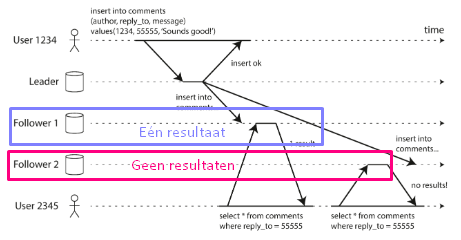
\includegraphics[width=\linewidth]{../images/Screenshot_213.png}
 	\caption{Het verschil tussen synchrone en asynchrone replication. Bij synchroon wacht je niet op bevestiging. Synchrone replicatie gaat direct door naar de target storage. Asynchrone replication wacht op bevestiging van de volgers op de source.}
\end{figure}

\subsubsection{Replicatiefouten}

Fouten bij synchrone replicatie zijn minder voorkomend, maar de techniek kan gedwarsboomd worden. Zo heb je nog steeds een probleem wanneer een write-operation niet kan worden afgewerkt als één van de volgers niet online is. Je wacht tot de bevestiging van de volgers.

\begin{figure}
	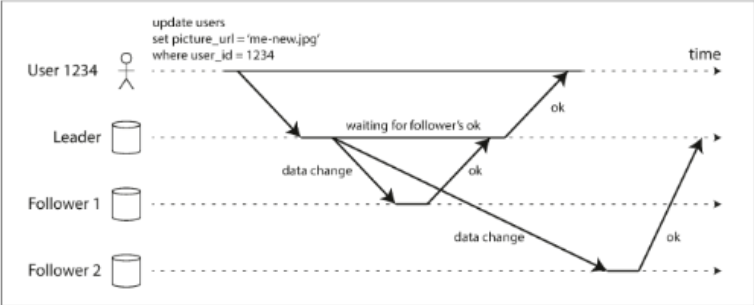
\includegraphics[width=\linewidth]{../images/Screenshot_160.png}
	\caption{Voorbeeld van een fout bij synchrone replicatie.}
\end{figure}

De twee vaak voorkomende fouten bij asynchrone replicatie zijn monotonic read en read-after-write. 

\begin{itemize}
	\item Read-after-write (RAW) duidt, zoals de naam het aangeeft, op een fout bij het lezen. De client heeft in dit geval een comment geplaatst en vervolgens wordt er een bevestiging gegeven aan de client. Daarna wilt dezelfde gebruiker dezelfde post inlezen, maar die is nog niet opgeslaan door een andere volger. Je wilt dezelfde output krijgen als je hetzelfde in de databank schrijft. Bij RAW is het belangrijk om met een timestamp te werken. Zorg dat je bij een schrijfoperatie alles tot aan een punt moet laten voldoen aan de timestamp. Zo ja, haal de gegevens op en geef ze aan de client. Zo niet, wacht of kijk naar een andere volger.
	\item Een gelijkaardig, maar nog steeds verschillend probleem, is monotonic read. De gebruiker leest een post of comment, maar na een refresh is deze comment opeens niet beschikbaar of niet-bestaand. De volger loopt hier achter op de andere volgers. De klok bij de ene volger loopt voor op de andere. Het verschil hier is dat de gebruiker de tekst niet heeft geschreven, wat wel het geval is bij RAW. Dit lossen we op door de gebruiker altijd van dezelfde replica te laten lezen. Hieronder leest de gebruiker eerst van de volger mét het resultaat. Daarna probeert de gebruiker dit opnieuw, maar bij een volger die achterloopt.
\end{itemize}


\begin{figure}
	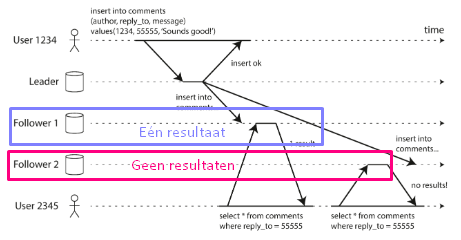
\includegraphics[width=\linewidth]{../images/Screenshot_213.png}
	\caption{Monotonic read}
\end{figure}

\begin{figure}
	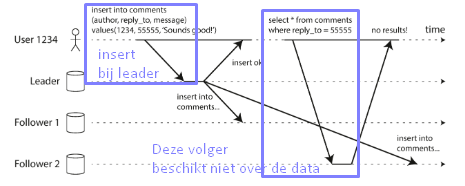
\includegraphics[width=\linewidth]{../images/Screenshot_214.png}
	\caption{Read-after-write probleem.}
\end{figure}

\subsection{Replicatie en partitionering combineren}

\begin{figure}
	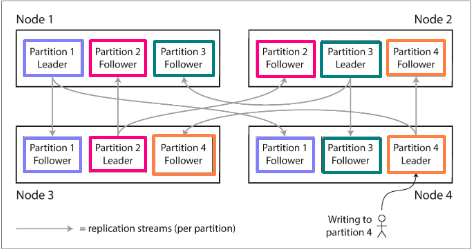
\includegraphics[width=\linewidth]{../images/Screenshot_215.png}
	\caption{Vier partities: elke leader heeft twee volgers. In de volgende foto zijn er vier nodes. Elke node heeft drie onderdelen. Over de vier nodes zijn er vier verschillende partities verdeeld. De replica's of volgers kan je achterhalen aan de hand van de stream. De leider van partitie 1 in node 1. De replica's zijn in Node 3 en in Node 4. De leider van partitie 2 is in node 3. De replica's zijn in Node 1 en in Node 2.}
\end{figure}

We kunnen niet zomaar data in stukken snijden. We moetne hotspots vermijden. Een hotspot is een plaats waar de verdeling geen goede verhouding heeft voor iedere node. Hiervoor hebben we twee oplossingen: key-value partitionering en hash partitionering.

\begin{itemize}
	\item Key-value partitionering is wanneer je een zo eerlijk en even mogelijke verdeling maakt over alle nodes. Alle sleutels binnen een node behoren tot een range. Je sorteert alle sleutels. Bijvoorbeeld alles van A t.e.m. E. Afhankelijk van de context wordt vaak voorkomende data binnen dezelfde partitie opgeslaan. Dit zorgt voor meer verkeer op partitie A-D vergeleken met X-Z. De ene partitie zal een hotspot worden, maar de andere zal geen verkeer krijgen.
	\item Hash partioning lost dit probleem merendeels op, maar het is niet de meest efficiënte implementatie. Hier verlies je sortering. De compromise hier is dat je wél een even verdeling zal krijgen. De hash houdt rekening met beschikbare plaats. De kans dat een partitie niet gebruikt zal worden is kleiner. 
\end{itemize}


\section{Request routing}

De plaats van data achterhalen kan op drie manieren:

1. Iedere node bevat metadata. De client kan een willekeurige knoop contacteren. De knoop weet waar het te zoeken woord is. Hieronder geeft knoop 0 mee dat het te zoeken woord op knoop 2 is.

2. Er is een laag tussen de client en de knopen. De routing-tier bevat metadata.

3. De client heeft directe toegang tot de metadata. Dit wordt het minste gebruikt.

\begin{figure}
	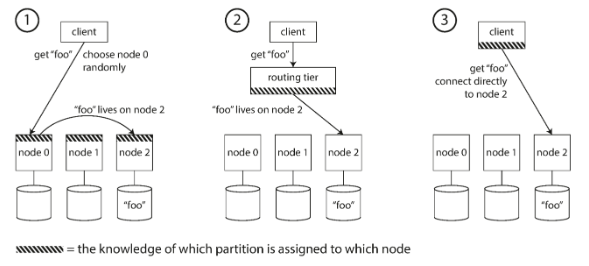
\includegraphics[width=\linewidth]{../images/Screenshot_216.png}
	\caption{De drie mogelijkheden om de plaats van data te achterhalen.}
\end{figure}

De locatie van metadata onderhouden gebeurt met de coordination service. Dit zorgt voor het onderhoud en de mapping van de metadata. Het is de routing tier (RT) tussen de client en de knopen. De RT is direct verbonden met zowel de knopen, alsook met de Zookeeper. Als er iets verandert in de data van een node, dan meoten de nodes dit laten weten aan de Zookeeper.

\begin{figure}
	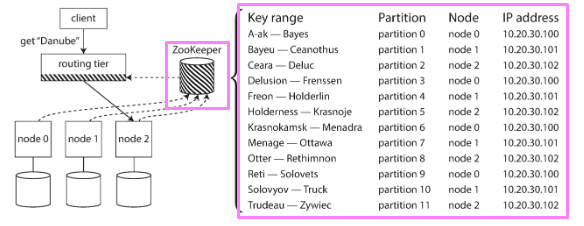
\includegraphics[width=\linewidth]{../images/Screenshot_217.png}
	\caption{Zookeeper.}
\end{figure}

\chapter{Hadoop Filesystem}

\section{Inleiding}

Het maakt gebruik van parallellisatie om de gegevens te verdelen over meerdere computers in een cluster, waardoor het verwerkingsproces sneller wordt. Dit kan worden gebruikt voor het analyseren van gegevens, zoals het ontdekken van trends en patroonherkenning. Hadoop is één van de eerste frameworks voor Big Data Processing. Het is een relatief oud project met *clunky* technieken. 

Het is ontworpen met de gedachten om clusters te kunnen draaien op normale hardware. Als je cluster bestaat uit honderden computers, dan is de kans groot dat er één zal breken. Het basisidee van Hadoop is om dit soort fouten af te handelen en zodat het systeem blijft werken zoals voordien.

\subsection{Hadoop stack}

Een pure hadoop-stack bestaat uit vier onderdelen:
* Hadoop common: de gedeelde bibliotheken die door de andere modules worden gebruikt. Je ziet dit gedeelte niet. Het is de meeste onderste laag.
* HDFS is een filesystem. Dit zorgt voor de distributed file storage. Je merkt de delay amper.
* MapReduce is het processing-gedeelte. MapReduce laat je toe om parallel grote datasets te verwerken.
* YARN voorkomt dat één element in je cluster alle resources opeet. Dit element zorgt voor request-afhandeling van resourcevragen.

\section{Hadoop filesystem}

\subsubsection{Algemeen}

Een filesystem laat toe om data op te slaan en weer op te halen. Er zijn drie soorten data: files, mappen en metadata. Metadata is de info over de mappen of bestanden, zoals file length en permissies. Een filesystem zorgt ervoor dat de data toegankelijk is. De consistentie in filesystems wordt bewaard door middel van een logsysteem. 

\begin{figure}
	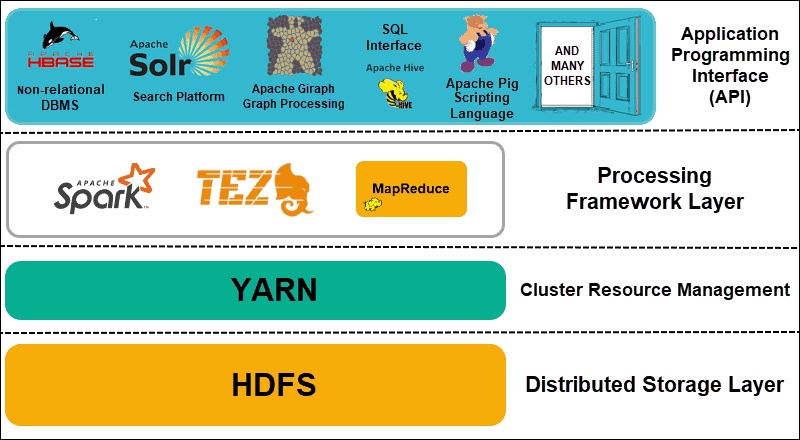
\includegraphics[width=\linewidth]{images/hadoop-ecosystem-layers.png}
	\caption{Het Hadoop ecosysteem. Onderaan staat Hadoop FileSystem. Daarboven is er YARN, wat instaat voor het resourcemanagement. Boven het filesystem en de resourcemanager staan er de processing services, waaronder Spark en MapReduce. API's komen in deze samenvatting niet aan bod.}
\end{figure}

\subsubsection{Designprincipes}

De data wordt opgeslaan in een cluster van gewone machines. De focus van HDFS ligt op riante hoeveelheden data op te slaan. Er wordt gewerkt met veel groepen van machines. Als er één machine zou kapot gaan, dan neemt een andere machine over. Er is weinig vertraging. Write-once-read-many-times (WORM) betekent dat gegevens één keer worden geschreven en vervolgens vele keren worden gelezen, maar niet wordt gewijzigd of verwijderd. HDFS ondersteunt deze techniek om zo een hoge fouttolerantie te kunnen bieden en doorvoer te kunnen bieden. Er zijn twee algemene redenen waarom er geen bestanden worden gewijzigd of verwijderd.

\begin{itemize}
	\item HDFS is bedoeld om grote hoeveelheden data op te slaan. Verwijderen en wijzigen vergt kostbare energie. Daarnaast is HDFS fouttolerant, want het systeem moet blijven werken zelfs al vallen er nodes uit. Als een bestand wordt verwijderd, dan beïnvloedt dit de integriteit van de data.
	\item HDFS is bedoeld om een historiek uit te bouwen. De data wordt ingezet in data-analyse, waar nauwkeurigheid een rol speelt, dus er mogen geen wijzigingen aan de data worden aangebracht.
\end{itemize}

Het principe is 'write-once, read-many-times'. Een bestand wordt eenmalig gemaakt. De doorvoer van het systeem is hier belangrijker. De hoeveelheid verwerkte data per tijdseenheid. HDFS op een klassiek filesysteem. Eens de machine bezig is kan je een grote doorvoer hebben. 

Er is sprake van \textbf{append-only fashion}. De gegevens kunnen enkel achteraan worden toegevoegd en niet tussenin of helemaal vooraan. Deze werkwijze helpt om de prestaties en betrouwbaarheid van HDFS te verbeteren, omdat het aantal wijzigingen aan gegevens beperkt. 

\subsubsection{Anti-patterns}

Er zijn enkele situaties waarbij HDFS \textit{overkill} of ongeschikt is als oplossing:

\begin{itemize}
	\item Wanneer snelheid een grote rol speelt. De latency is hier niet minimaal.
	\item Wanneer het merendeel van de data uit kleine bestanden bestaat. De nadruk bij HDFS ligt op grote bestanden. De NameNode houdt de directorystructuur bij, waardoor veel kleine bestanden zal leiden tot veel verschillende takken.
	\item Wanneer je meerdere schrijvers op eenzelfde moment wilt hebben. Als één client schrijft en de andere wilt lezen, dan kan er een conflict ontstaan bij de integriteit en het delen van een bestand.
	\item Wanneer je gegevens
\end{itemize}

* Append-only fashion: Als je inhoud vooraan of in het midden wilt toevoegen.


\section{Hadoop-onderdelen}

HDFS heeft twee componenten:

\begin{itemize}
	\item De NameNode.
	\item De DataNode.
\end{itemize}

Kort samengevat is de namenode de node dat het bestandssysteem beheert en bijhoudt waar alle bestanden zijn opgeslagen. De datanode slaat de bestanden op en zorgt ervoor dat gegevens beschikbaar zijn voor lezen en schrijven.

\subsection{NameNode}

Een NameNode (NN) is de centrale coördinator. weet uit welke blokken de data bestaat en houdt bij op welke datanodes de blokken staan. Locaties worden niet persistent bijgehouden. Onderling weten ze dit door middel van \textit{heartbeats}.  Als je een file wilt hernoemen, dan lukt dat ook. Bij een cluster heb je altijd één NN.

De NN heeft de volgende rollen:

\begin{itemize}
	\item Het beheerde de filesystem namespace.
	\item Het koppelt de datablokken aan de DataNodes.
	\item Het handelt de filesystemverzoeken, zoals het openen/sluiten en hernoemen van bestanden of mappen.
	\item Het gidst de client naar de best passende DataNode.
\end{itemize}

\subsubsection{Opslag voor metadata}

De NameNode slaat metadata over het filesystem op in twee bestanden: de namespace image en de edit log. De \textit{namespace image} bevat informatie over de structuur van het filesystem (metadata), waaronder de directoryboom en de bestanden en mappen die het bevat. De metadata wordt in het RAM bijgehouden. Daarmee is het snel, maar vluchtig. Terwijl het systeem loopt wordt het opgebouwd, maar de informatie is niet persistent. 

De \textit{edit log} bevat een opname van alle wijzigingen in het filesystem, zoals het maken of verwijderen van bestanden en mappen. Dit is een append-log. Telkens als er iets verandert, dan wordt er informatie toegevoegd. Als de NN opnieuw zou opstarten, dan wordt de image en edit log gelezen. Daarna worden de veranderingen van de edit log toegepast op de namespace image om zo een nieuwe namespace image te maken. Daarna wordt een nieuwe edit log gestart.

\subsubsection{Werking NameNode}

De NameNode communiceert met de DataNodes om bij te houden op welke DataNodes welke datablokken worden opgeslagen. Daarnaast zorgt de NN ervoor dat de data beschikbaar en consistent is over een cluster. Wanneer een client data in HDFS wil raadplegen, stuurt hij een verzoek naar de NameNode, die vervolgens bepaalt op welke DataNode de gevraagde datablok staat en de client naar die DataNode stuurt.

\subsection{DataNode}

De DataNodes (DN) stellen de servers voor die de werkelijke datablokken opslaan. Ze zijn verantwoordelijk voor het afhandelen van lees- en schrijfverzoeken voor het maken/verwijderen en hermaken van datablokken. Deze acties gebeuren volgens de instructies van de NN. Alle instructies worden gegeven met een \textit{block report}, wat een periodieke rapportering is van de NN.

Een DN heeft de volgende functies:

\begin{itemize}
	\item Direct luisteren naar instructies van de NN.
	\item Lees- en schrijfverzoeken afhandelen.
	\item Het maken, verwijderen of repliceren van datablokken.
\end{itemize}

Een DN is het werkpaard van een HDFS-cluster, want ze beheren en slaan de data op die in een cluster kan worden teruggevonden. In het werkveld zijn er riante hoeveelheden DN's aanwezig. Alles wat de client leest is afkomstig van een DN. Elk blok heeft een replicatiefactor. De replicatiefactor wijst op hoeveel systemen het bestand beschikbaar moet staan. Een HDFS heeft veel DataNodes.

\subsubsection{Werking DataNode}

Wanneer een client data in HDFS wil raadplegen, stuurt hij een verzoek naar de NameNode, die vervolgens bepaalt op welke DataNode de gevraagde datablok staat en de client naar die DataNode stuurt. De DataNode haalt vervolgens de gevraagde datablok op en stuurt deze terug naar de client.

\begin{figure}
	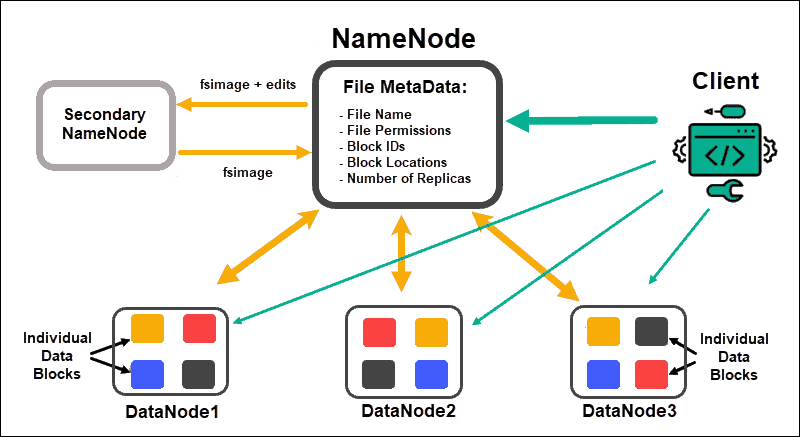
\includegraphics[width=\linewidth]{images/hdfs-components-namenode-datanode-datanode.png}
	\caption{De verschillende componenten van HDFS, waaronder DataNodes en NameNodes.}
\end{figure}

\section{Single-point-of-failure}

Als één NN uitvalt, of als de NS Image uitvalt, dan zullen de datablokken niet meer toegankelijk zijn. Alle data zal wél blijven bestaan op de DN. Alle blokken hebben random verwijzingen. Als client ben je er niet van bewust waarvan de data komt en waartoe die gaat. 

\subsection{Bescherming NameNode}

Er zijn twee manieren om het NN te beschermen:

\begin{itemize}
	\item De meest voor de hand liggende manier is om regelmatig een backup te nemen. Hadoop kan worden geconfigureerd om metadata op meerdere filesystems op een synchrone en atomaire manier te schrijven. 
	\item De tweede optie is een secondary NN. Zolang je een systeem niet herstart wordt je edit log langer en groter. Dit is niet ideaal, want als het neemt zowel plaats in alsook zal het opstarten van een NS image langer duren. In latere versie van Hadoop hebben ze een secondary NN toegevoegd. Een secondary NN is een proces dat op een andere computer loopt en dat de veranderingen van de edit log verwerkt in de huidige namespace.
\end{itemize}}

\section{HDFS Blokken}

Datablokken hebben niets te maken met "blokken" op een traditionele harde schijf. De datablokken op een Hadoop FS verwijzen naar de stukken data waarin een bestand wordt verdeeld voor opslag. De standaardgrootte van een bestand is 128MB, dus relatief groot. Door een bestand in blokgroottet te verdelen, kan het in HDFS worden opgeslagen, zelfs als het groter is dan elke enkele schijf in een cluster. Het laatste blok van een bestand kan kleiner zijn dan de standaardblokgrootte als het bestand niet een exact veelvoud is van de blokgrootte.

\subsubsection{Preventie}

Om dataverlies te voorkomen, wordt voor elk bestand in HDFS een replicatiefactor ingesteld. Deze waard steld het aantal replicants voor. Een replicant is een 'dubbel' van een bestand. HDFS zal \textit{proberen} om het aantal replicanten te laten overeenkomen met de opgestelde replicatiefactor. Verschillende bestanden kunnen afwijkende replicatiefactoren hebben. De factor hangt af van de gewenste redundantie en bescherming.

\section{Anatomy}

\subsection{Anatomy of a File Read}

Het proces om een bestand uit HDFS te lezen, omvat de volgende stappen:

\begin{enumerate}
	\item De Client maakt een oproep naar een instantie van het HDFS.
	\item De instantie maakt gebruik van Remote Procedure Calls (RPC) naar de NN om de lcoaties van de eerste paar blokken in het bestand te achterhalen. Voor elke blok geeft de NN de adressen van de DN's die een kopie hebben van dat blok. Die adressen zijn gesorteerd op afstand van de DN tot de client. De HDFS geeft een \textit{DataInputStream}-object terug naar de client. Dit object bevat een \textit{DFSInputStream}-object, die de Input/Output tussen de DN en de NN beheert.
	\item De client roept een leesoperatie op de stream. Het \textit{DFSInputStream}-object verbindt automatisch met de DN voor de volgede blok. Dit gebeurt transparant met de client, wie denkt dat het een continue stream aan het lezen is. 
	\item Eenmaal de client klaar is met lezen, dan stuurt de client een een \textit{close} op de \textit{FSDataInputStream}.
\end{enumerate}

De client contacteert de DN direct om data op te halen. De NN gidst de client richting de meest optimale verbinding met een datablok. De NN geeft géén data, maar het verleent enkel richting door de locaties van de block requests terug te geven. Deze locaties staan in het RAM-geheugen, daarom gebeurt dit proces heel snel.

\subsubsection{Rollen}

\begin{itemize}
	\item De \textit{DistributedFileSystem} is een Java-klasse die een interface voorziet om met het HDFS te kunnen interrageren. Met dit interface kan een client toegang tot een bestand krijgen of een bestand manipuleren. De DFS communiceert met de NN om acties uit te voeren. De DFS gebruikt RPC's om verzoeken naar de NN te versturen en te ontvangen. De meest gebruikte functies zijn: 
	\begin{itemize}
		\item 'open' om een bestaand bestand te openen: een inputstream wordt teruggegeven.
		\item 'create' om een nieuw bestand aan te maken: een outputstream wordt teruggegeven om data in het bestand te schrijven
		\item 'delete' om een bestand te verwijderen
		\item 'mkdirs' om een nieuwe directory te maken
		\item 'listStatus' om een lijst van bestanden en directory statussen, van een gespecifeerd pad, terug te krijgen
	\end{itemize}
	\item De DFSInputStream is een interne klasse dat gebruikt wordt om data uit een bestand te lezen. Het verbindt met het passende DN, daarnaast streamt het de data terug naar de client.
	\item De DataInputStream is een klasse dat een interface voorziet om datatypes uit te lezen. Het wordt gebruikt om data van eender welke inputstream te lezen, inclusief een DFSInputStream.
	\item Een FSDataInputStream is een klasse die de DFSInputStream inkapselt en extra functionaliteit aanbiedt. Het wordt gebruikt om eender welke data te lezen van een bestand in HDFS.
\end{itemize}


\begin{figure}
	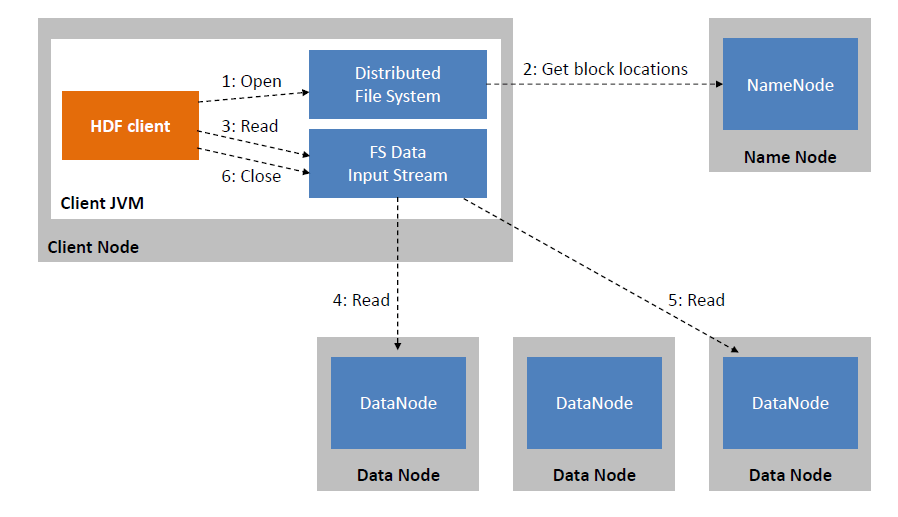
\includegraphics[width=\linewidth]{images/HDFS-Read.png}
	\caption{File read schema opgehaald van Javatpoint (2022)}
\end{figure}

\subsection{Anatomy of a File Write}

Het proces om een nieuw bestand in HDFS te maken, omvat de volgende stappen:

\begin{enumerate}
	\item De client roept een \textit{create} of \textit{delete} aan op de \textit{DistributedFileSystem}.
	\item Het HDFS maakt een RPC-oproep om een nieuw bestand in de namespace van het filesystem te maken, zonder blokken die eraan gekoppeld zijn. De NN voert controles uit, waaronder kijken of het bestand bestaat of kijken naar de machtigingen van de client. Als alle controles slagen, dan maakt de NN een record van het nieuwe bestand. Zo niet, dan faalt de \textit{file creation} en dan krijgt de client een \textit{IO-exception} te zien.
	\item Het HDFS geeft een \textit{FSDataOutputStream} terug aan de client. Dit object bestaat uit een \textit{DFSOutputStream}, die de communicatie met de DN's en de NN beheerst.
	\item Als de client gegevens schrijft, dan wordt de \textit{DFSOutputStream} in pakketten gesplitst. Deze pakketten worden naar een \textit{data queue} geschreven. Deze wachtrij wordt doorgestuurd naar een \textit{DataStreamer}. Dit object vraagt om beurt aan de NN om nieuwe blokken te alloceren, dit met een lijst van geschikte DN's om de replicaties op te slaan.
	\item De lijst van DN's vormt een pipeline.
	\item Het \textit{DataStreamer}-object streamt de pakketten naar de eerste DN in de pipeline, die elk pakket opslaat en doorstuurt naar de tweede DN in de pipeline. De tweede DN herhaalt dit, de derde DN herhaalt dit, enzovoort.
	\item De \textit{DFSOutputStream} onderhoudt een \textit{acknowledgement queue}. Dit terwijl pakketten worden bevestigd door de DN's. De pakketten worden van de \textit{ack queue} verwijderd als ze door alle DN's in de pipeline zijn bevestigd.
	\item Eenmaal de client klaar is met het schrijven van gegevens, roept de client \textit{close} aan op de stream. Dit spoelt alle overblijvende pakketten naar de DN-pipeline en wacht op bevestigingen voordat hij contact opneemt met de NN. De NN weet al uit welke blokken het bestand bestaat, dus deze node moet enkel wachten tot de blokken gerepliceerd zijn voordat de node succesvol terugkomt.
\end{enumerate}

\subsubsection{Rollen}
\begin{itemize}
	\item De \textit{DistributedFileSystem} is een Java-klasse die een interface voorziet om met het HDFS te kunnen interrageren. Met dit interface kan een client toegang tot een bestand krijgen of een bestand manipuleren. De DFS communiceert met de NN om acties uit te voeren. De DFS gebruikt RPC's om verzoeken naar de NN te versturen en te ontvangen. De meest gebruikte functies zijn: 
	\begin{itemize}
		\item 'open' om een bestaand bestand te openen: een inputstream wordt teruggegeven.
		\item 'create' om een nieuw bestand aan te maken: een outputstream wordt teruggegeven om data in het bestand te schrijven
		\item 'delete' om een bestand te verwijderen
		\item 'mkdirs' om een nieuwe directory te maken
		\item 'listStatus' om een lijst van bestanden en directory statussen, van een gespecifeerd pad, terug te krijgen 
	\end{itemize}
	\item De \textit{DataStreamer} is verantwoordelijk voor het streamen van data vanuit de client naar de verschillende DN's in een cluster. Het wordt gebruikt wanneer een gebruiker wilt schrijven naar een bestand in een HDFS. Dit object vraagt de blokallocaties aan de NN, zo wordt er een lijst bijgehouden van geschikte DN's.
	\item Een \textit{DFSOutputStream} is een interne klassie die gebruikt wordt om data te schrijven naar een bestand. Het splitst de data in pakketten, streamt de pakketten naar de DN's en verzekert dat de data op een betrouwbare manier wordt afgehandeld.
	\item De \textit{FSOutputStream} is een publieke lasse dat een interface voorziet voor clients om data uit te schrijven naar een bestand in een HDFS. Het inkapselt de \textit{DFSOutputStream} en synchroniseert de data stream.
\end{itemize}


\begin{figure}
	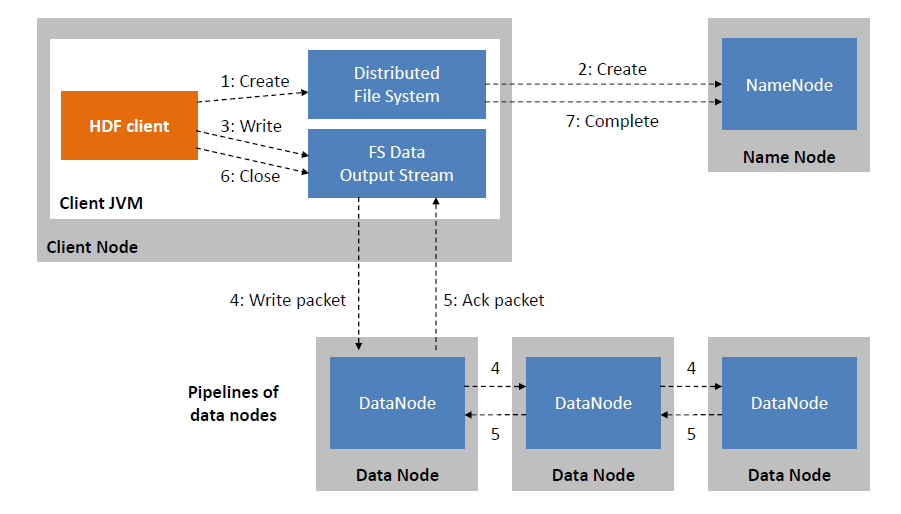
\includegraphics[width=\linewidth]{images/HDFS-Write.png}
	\caption{File Write schema opgehaald van Javatpoint (2022)}
\end{figure}

\subsubsection{Foutafhandeling}

Bij het falen van een DN, terwijl er data naartoe wordt geschreven, dan worden er enkele acties afgehandeld. De client weet wat er achter de schermen gebeurt bij zo een afhandeling. Sommige blokken kunnen \textit{under-replicated} zijn, maar de NN zal dit opmerken. De blokken zullen asynchroon worden gerepliceerd in de cluster. Dit proces herhaalt zich tot de replicatiefactor is behaald.

\section{Command-Line}

De CLI voor HDFS biedt een reeks commando's aan om te communiceren met een HDFS-cluster. Deze taal heeft gelijkenissen met de Bash-taal. Om een lijst te krijgen met beschikbare commando's en opties, kan je het commando "hadoop fs -help" gebruiken.

\subsubsection{Kopiëren en ophalen}

\begin{lstlisting}[language=Hadoop]
// Lokaal --> HDFS
hadoop fs --copyFromLocal input/docs.txt hdfs://localhost/user/dylan/docs.txt

// Alles in een Hadoop map bekijken
hadoop fs -ls .

// HDFS naar Lokaal
hadoop fs --copyToLocal hdfs://localhost/user/dylan/docs.txt output/docs.txt
\end{lstlisting}

\subsubsection{Nieuwe elementen aanmaken}
\begin{lstlisting}
// Bestand aanmaken
hadoop fs -touch docs.txt

// Directory aanmaken
hadoop fs -mkdir input
\end{lstlisting}

\section{MapReduce}

Hadoop MapReduce is een programma dat wordt gebruikt voor het verwerken van grote hoeveelheden gegevens in een distributiefile-systeem. Het maakt gebruik van parallellisatie om de gegevens te verdelen over meerdere computers in een cluster, waardoor het verwerkingsproces sneller wordt. Dit kan worden gebruikt voor het analyseren van gegevens, zoals het ontdekken van trends en patroonherkenning. Een MapReduce bestaat uit drie fasen:

\begin{enumerate}
	\item Mapping
	\item Shuffle
	\item Reduce
\end{enumerate}

\subsubsection{Voordelen van MapReduce}

MapReduce vereist geen kennis van parallelisatie, data distributie en fouttolerantie binnen het programmeren. Dit gebeurt automatisch over een riant aantal machines gespreid. Alle details rond partitionering van de input-data, scheduling en foutafhandeling wordt al afgehandeld. Bij MapReduce kan de programmeur focussen op de logica van de applicatie en het is zo makkelijker om parallele programma's te schrijven die schaalbaar, efficiënt en fouttolerant zijn. Bij MapReduce is \textit{re-execution} het belangrijkste mechanisme. Als een taak faalt, dan zal het framework automatisch de taak opnieuw proberen op een nieuwe machine.

\subsection{Data Flow}

 Het framework zal iedere split aan een \textit{map task} toekennen. Deze task

\begin{enumerate}
	\item Bij een MapReduce job wordt de inputdata over verschillende \textit{chunks} of \textit{inputsplits} heen verdeeld. De \textit{map job} zal het deel lijn per lijn bekijken. Iedere mapper zal een deel van het bestand te zien krijgen.
	\item Het framework zal iedere split aan een \textit{map task} toekennen. De \textit{map task} verwerkt de data en genereert een set van key-value paren.
	\item Het framework verzamelt en groepeert de waarden met dezelfde key. Deze groeperingen worden doorgegeven aan de \textit{reduce task}.
	\item De \textit{reduce task} verwerkt de keys met hun waarden. De output is een verzameling van key-value paren. Deze output wordt naar een outputbestand in HDFS geschreven.
\end{enumerate}

\subsection{Mapping}

De Mapper in Hadoop MapReduce is een programma dat wordt gebruikt om gegevens te verdelen over meerdere computers in een cluster, zodat ze parallel kunnen worden verwerkt. De Mapper leest de gegevens in en verdeelt ze in kleinere stukjes, die vervolgens naar de verschillende computers in het cluster worden gestuurd om te worden verwerkt. Dit maakt het mogelijk om grote hoeveelheden gegevens snel te verwerken en te analyseren. De Mapper is het eerste onderdeel van het MapReduce-proces en zorgt ervoor dat de gegevens op een gestructureerde manier worden verwerkt.

\subsubsection{Voorbeeld luchttemperatuur}

De mapfunctie zal ieder inputrecord verwerken. Ieder record bestaat uit lijnen tekst. Bij het verwerken worden de jaar- en luchttemperatuurvelden uit het bestand gehaald. Het filter recors met ontbrekende of verdachte temperaturen. De mapfunctie zal key-value paren voor ieder record gaan genereren. De key is het jaar en de value is de luchttemperatuur. De mapfunctie geeft de key-value paren aan de shuffle \& sort fase.

\subsection{Shuffling}

De Shuffle-fase in Hadoop MapReduce is een belangrijk onderdeel van het MapReduce-proces waarbij de gegevens worden verzameld en gerangschikt op basis van de sleutels die aan de gegevens zijn toegekend. De Mapper verdeelt de gegevens in kleinere stukjes en stuurt deze naar de verschillende computers in het cluster, waar ze worden verwerkt. De Reducer verzamelt vervolgens de verwerkte gegevens van alle computers in het cluster en sorteert ze op basis van de sleutels, zodat de gegevens kunnen worden verwerkt en geanalyseerd. De Shuffle-fase is dus een cruciale stap in het MapReduce-proces omdat het ervoor zorgt dat de gegevens op een gestructureerde manier worden verwerkt en geanalyseerd.

\subsection{Reduce}

In een MapReduce job zal de input van de reducefunctie uit key-value paren bestaan. Die werden aangemaakt door de mapfunctie en doorgegeven aan de shuffle \& sort fase. De reducefuntie verwerkt iedere key met de toebehorende waarden. Uiteindelijk is de laatste stap in de MapReduce om een output te maken. De reducer wordt bijvoorbeeld gebruikt om totale aantallen te berekenen of gemiddelden te berekenen voor een bepaalde groep gegevens. Het is een belangrijk onderdeel van het MapReduce-proces omdat het ervoor zorgt dat de gegevens op een gestructureerde manier worden verwerkt en geanalyseerd.


\subsubsection{Voorbeeld luchttemperatuur}

De reducefunctie zal, van de shuffle \& sort fase, een verzameling van key-value paren ontvangen. De key is hier het jaar, en de value is de luchttemperatuur. De reducefunctie itereert door de temperatuurwaarden van ieder jaar en het neemt de maximale waarde. Dit hoort tot de finale uitvoer. De finale uitvoer bestaat uit een set key-value paren, waarbij de key het jaar is en de waarde de grootste luchttemperatuur die werd opgenomen in dat jaar.

\section{Java MapReduce}

Java werd gekozen omdat dit de meest prevalente taal is voor MapReduce. Een MapReduce applicatie bestaat uit drie onderdelen:

\begin{enumerate}
	\item Het schrijven van de mapfunctie. De mapfunctie zal iedere input record verwerken en maakt hierop een verzameling van key-value paren. De mapper-klasse wordt ge-\textit{extend} en enkel de \textit{map()}-methode wordt overerfd. De \textit{map()}-methode vraagt een sleutel als inputwaarde op. Dit is regelmatig de lijn waarop tekst voorkomt. Op basis van deze invoer maakt het een verzameling van key-value paren.
	\item Het schrijven van de reducefunctie. De reducefunctie verwerkt iedere key met de toebehorende waarden. Je moet de Reducer-klasse \textit{extenden} en de \textit{reduce()}-methode overerven. De input bij deze methode is een sleutel en een set waarden dat de verzameling van output key-value paren gaat maken.
	\item Boilerplate-code schrijven. Dit is de code die specifieert hoe de MapReduce job moet draaien. Iedere fase, inclusief extra-reduce fasen, moeten aan bod komen. Alles van job configuratie, input en outputpaden instellen en \textit{job running} moet in de boilerplate code terug te vinden zijn. 
	\item In sommige gevallen kan je ook een combinerfunctie schrijven. Deze gelijkt sterk op een reducefunctie en wordt op de output van de \textit{map task} toegepast. De combinerfunctie wordt gebruikt om het aantal data, dat tussen de mapper en de reducer bevindt, aan te passen. Zo wordt het proces efficiënter behandeld. Voor een combiner moet je de Reducer-klasse \textit{extenden} en de \textit{reduce()}-methode overerven, net zoals bij de reducefunctie.
\end{enumerate}

\begin{figure}
	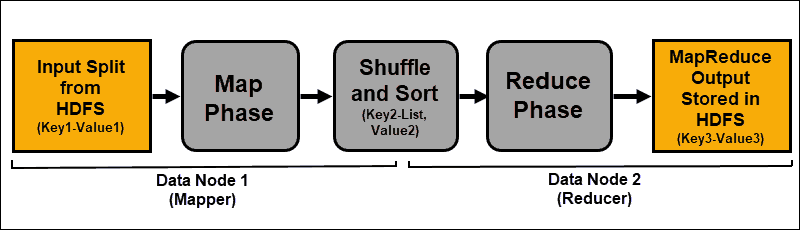
\includegraphics[width=\linewidth]{images/mapper-reducer-mapreduce-job-flow.png}
	\caption{Een vereenvoudigde versie van de job-flow bij MapReduce.}
\end{figure}

\subsubsection{WordCount-oefening}

\begin{lstlisting}[language=Java]
public class WordCount {
	
	public static class TokenizerMapper
	extends Mapper<Object, Text, Text, IntWritable>{
		
		private final static IntWritable one = new IntWritable(1);
		private Text word = new Text();
		
		public void map(Object key, Text value, Context context
		) throws IOException, InterruptedException {
			StringTokenizer itr = new StringTokenizer(value.toString());
			while (itr.hasMoreTokens()) {
				word.set(itr.nextToken());
				context.write(word, one);
			}
		}
	}
	
	public static class IntSumReducer
	extends Reducer<Text,IntWritable,Text,IntWritable> {
		private IntWritable result = new IntWritable();
		
		public void reduce(Text key, Iterable<IntWritable> values,
		Context context
		) throws IOException, InterruptedException {
			int sum = 0;
			for (IntWritable val : values) {
				sum += val.get();
			}
			result.set(sum);
			context.write(key, result);
		}
	}
	
	public static void main(String[] args) throws Exception {
		Configuration conf = new Configuration();
		Job job = Job.getInstance(conf, "word count");
		job.setJarByClass(WordCount.class);
		job.setMapperClass(TokenizerMapper.class);
		job.setCombinerClass(IntSumReducer.class);
		job.setReducerClass(IntSumReducer.class);
		job.setOutputKeyClass(Text.class);
		job.setOutputValueClass(IntWritable.class);
		FileInputFormat.addInputPath(job, new Path(args[0]));
		FileOutputFormat.setOutputPath(job, new Path(args[1]));
		System.exit(job.waitForCompletion(true) ? 0 : 1);
	}
}
\end{lstlisting}

\subsection{Mapper-klasse}

De mapperklasse is een generieke klasse dat vier typeparameters heeft. De mapfunctie zal bij ieder input record een verzameling key-value paren aanmaken. Hier zal de key het regelnummer zijn. De value zal de toebehorende tekst op de regel zijn.
\begin{itemize}
	\item De input key type is een Object.
	\item De input value type is een Text.
	\item De output key type is een Text. Dit is de volledige tekst dat op een lijn terug te vinden is. representeert het woord waarop er geteld word.
	\item De output value type is een IntWritable. Dit is het aantal voorkomens van het toebehorende woord.
\end{itemize}

\subsection{Reduce-klasse}

De reduceklasse verwerkt iedere key en de toebehorende waardeN. De outputkey zal hier het woord zijn, en de outputvalue zal hier het aantal voorkomens van een woord in een bestand zijn. 

\subsection{Main-methode}

De main-methode zal een Job-object aanmaken. Dit object geeft aan hoe de job moet worden gedraaid. De \textit{setJarByClass}-methode specifieert het JAR-bestand dat de klassen bevat in de job. Hadoop gebruikt deze informatie om het meest passende JAR-bestand terug te vinden. Vervolgens worden de input- en outputpaden toegelicht. 

\subsubsection{Inputpaden}
Het inputpad wordt bepaald door \textit{addInputPath} van het object \textit{FileInputFormat}. De input kan hier één bestand, maar ook meerdere bestanden in een directory zijn. Globbing is ook mogelijk.

\subsubsection{Outputpaden}

Het outputpad wordt bepaald door \textit{addOutputPath} van het object \textit{FileOutputFormat}. De outputfile of directory mag, voor het uitvoeren van de job, niet bestaan! Deze voorzorg wordt genomen om \textit{data loss} te voorkomen.

\subsubsection{Afwerking}

De \textit{waitForCompletion}-methode wacht tot de job is afgerond. Bij het al dan niet succesvol afwerken zal de job een boolean teruggeven. 

\subsection{Development Environment}

\subsubsection{POM-file}
Alle projecten worden van het formaat 'Maven' zijn. Dit wordt vlot in Eclipse aangemaakt. De \textit{dependencies} moeten de nodige MapReduce en Hadoop plugins bevatten. Alle dependencies kan de ontwikkelaar terugvinden in het \textit{pom.xml} bestand. Dit bestand is het configuratiebestand van Maven.

\subsubsection{JAR genereren}

Om te kijken of alle dependencies en properties correct zijn ingesteld, moet de ontwikkelaar een JAR maken. Dit door te rechtermuisklikken op de POM-file, vervolgens moet een nieuwe build worden aangemaakt.  In de uitvoer krijgt de ontwikkelaar een \textit{build failure} of een \textit{build success}.

\subsubsection{JAR in een Hadoop NameNode plaatsen.}

Het JAR-bestand wordt in de vagrantmap geplaatst. Er wordt verondersteld dat de Hadoop-container aan het draaien is. De JAR-file wordt naar een NN-cluster doorgestuurd met de volgende commando's.

\begin{lstlisting}[language=Bash]
// op de vagrantmachine
docker cp target/hadoop-example-1.0-SNAPSHOT.jar namenode:/
docker exec -it namenode bash
ls -l hadoop-example-1.0-SNAPSHOT.jar

// in de hadoop-shell
hadoop fs -mkdir input/ncdc
hadoop fs -copyFromLocal 190? input/ncdc
hadoop fs -ls input/ncdc

// het uitvoeren van de JAR in de hadoop-shell
hadoop jar hadoop-example-1.0-SNAPSHOT.jar be.hogent.dit.tin.MaxTemperature input/ncdc output/ncdc

// resultaat bekijken
hadoop fs -cat output/ncdc/part-r-00000
\end{lstlisting}

\section{YARN}

\subsection{Algemeen}

YARN is een resourcemanager voor Hadoop-clusters. Deze daemon onderhoudt het toewijzen van CPU, geheugen en middelen aan verschillende toepassingen die op de cluster draaien. YARN biedt API's om mideelen op een cluster te verzoeken te gebruiken, maar deze API's worden niet door de gebruiker gebriukt. In plaats daarvan schrijven gebruikers naar \textit{higher-level} API's die door \textit{distributed computing frameworks} worden aangeboden. Voorbeelden hiervan zijn: MapReduce, Spark en Flink. Deze high-level API's verbergen de details van resourcemanagers. Zo kunnen programmeurs focussen op de logica.

\subsubsection{Extra ondersteuning}

YARN biedt ook ondersteuning voor het inplannen en uitvoeren van toepassingen op de cluster, alsook het monitoren van de status van die toepassingen. Gebruikers kunnen zo een groot aantal toepassingen uitvoeren op deen Hadoop-cluster, waaronder \textit{batch processing}, \textit{stream processing}, \textit{machine learning} en \textit{interactive SQL}.

\subsection{Core Services}

YARN biedt \textit{core services} aan van twee types \textit{long-term daemon processes}: 

\begin{itemize}
	\item Er is slechts één resourcemanager (RM) per Hadoop-cluster. Deze is verantwoordelijk voor het beheren van middelengebruik per cluster. De RM ontvangt \textit{resource requests} van \textit{application masters} en bepaalt vervolgens welke nodes op de cluster beschikbare middelen hebben om deze verzoeken te vervullen.
	\item Er is één actieve nodemanager (NM) op elke node van een Hadoop-cluster. De NM is verantwoordelijk voor het monitoren en opstarten van de containers op een node. Een container is een \textit{ligth-weight execution environment} die een toepassingsspecifiek proces uitvoert met een beperkt aantal middelen, zoals geheugen en CPU. Containers in YARN zijn niet gerelateerd aan de containers dat Docker heeft.
\end{itemize}

De RM en NM werken samen om middelen toe te wijzen en applicaties uit te voeren op een Hadoop-cluster. Gebruikers kunnen hun toepassingen aan YARN voorstellen via high-level API's.

\begin{figure}
	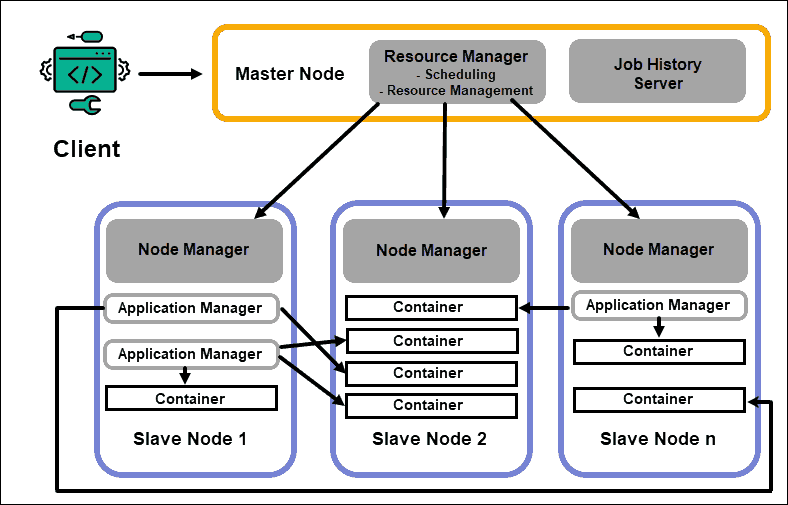
\includegraphics[width=\linewidth]{images/yarn-daemons-hadoop-architecture.png}
	\caption{YARN architectuur met daemon services.}
\end{figure}

\subsection{YARN Application run}

\begin{enumerate}
	\item Een client neemt contact op met de RM en vraagt om een \textit{application-master-process} op te starten.
	\item De RM zoekt een NM die de \textit{application-master} in een contianer kan starten. Alles daarna is afhankelijk van de toepassing. Bij een berekening moet er een waarde naar de client worden teruggestuurd. Bij MapReduce moet er een gedistribueerde bewerking worden uitgevoerd, want alle woorden zijn verspreid over verschillende containers. YARN zelf biedt géén manier om onderdelen van een toepassing met elkaar te laten communiceren.
\end{enumerate}

\subsection{Resource requests}

In een YARN resourcemanager wordt een resource request verstuurd om een specifieke taak mogelijk te maken. Deze request bevat een gepast aantal bewerkingsmiddelen, zoals CPU en geheugen. Deze requests bevatten \textit{locality constraints}. Dit geeft aan waartoe de middelen moeten beschikbaar worden gesteld. Als een container een HDFS blok moet verwerken, dan moet de resource request toelichten dat een container op één van de nodes, waar er een replica is, moet worden geplaatst. Zo wordt de data doorvoer geminimaliseerd én de snelheid van de applicatie wordt verbeterd.

\subsection{Scheduling}

De scheduler bepaalt of de middelen beschikbaar zijn en, indien mogelijk, worden de middelen toegekend aan de toepassing. Als een cluster druk is, met andere woorden zijn de middelen niet direct beschikbaar, dan zal de scheduler de \textit{resource requests} tijdelijk \textit{on-hold} plaatsen. Nadien worden de middelen aan de applicatie toegekend.

\subsubsection{Verschillende schedulers}

Er zijn verschillende schedulers in YARN:

\begin{itemize}
	\item FIFO, of \textit{first-in, first-out} zal de middelen aan applicaties toekennen in de volgorde waarin de scheduler de request kreeg. \textit{First come, first served}.
	\item \textit{Capacity scheduler} laat administrators toe om specifieke middelen te reserveren voor gepaste types toepassingen. 
	\item \textit{Fair scheduler} zal de resources op een eerlijke manier proberen te verdelen over alle applicaties heen. Hier zijn er verschillende factoren zoals de noden aan middelen en voorafgaand gebruik voor iedere applicatie.
\end{itemize}

\chapter{Spark}

\subsubsection{Vooraf}

Voor de komst waren er een aantal programmeermodellen gericht op filesystemclusters. De meeste waren gespecialiseerd, waaronder MapReduce, Storm, Impala en Pregel. Spark werd ontworpen om sneller en flexibeler te zijn dan de vooraf genoemde modellen. Sindsdien is het een populaire keze geworden voor een heleboel dataverwerkingstaken, waaronder \textit{batch processing}, streamverwerking, \textit{machine learning} en gegevensanalyse. Het biedt een aantal voordelen t.o.v. andere clustercomputersystemen, zoals: 

\begin{itemize}
	\item Flexibele en expressieve API
	\item Ondersteuning voor een breed aantal gegevensbronnen en formaten
	\item Mogelijk om te draaien in een groot aantal deployment-omgevingen, zoals on-premises clusters, cloudgebaseerde clusters en zelfs op één enkele machine.
\end{itemize}

\subsubsection{Algemene voordelen}

Spark is generiek en algemeen. Een analoge uitleg is om Spark een smartphone te noemen, terwijl andere modellen eerder een GPS, mobiele telefoon of digitale camera zijn. Spark is een \textit{jack-of-all-trades}. daarom brengt het drie voordelen met zich mee:

\begin{itemize}
	\item Toepassingen zijn makkelijker te ontwikkelen, want ze maken gebruik van een gecentraliseerde API.
	\item Het is efficiënter om verwerkingstaken te combineren. Voor Spark moeten pipelines vaak de gegevens wegschrijven naar opslag om ze door te geven aan een andere engine. Spark kan diverse functies uitvoeren op dezelfde gegevens, vaak in het geheugen.
	\item Spark maakt nieuwe toepassingen mogelijk, bijvoorbeeld interactieve queries op het streamen van ML.
\end{itemize}

\section{Spark Application Architecture}

Er zijn drie belangrijke rollen:

\begin{itemize}
	\item Bij een Spark-applicatie is de \textit{driverprocess} hetgeen wat de applicatiecode doet draaien. Dit proces onderhoudt de informatie van de Spark-applicatie, beantwoordt de input van de gebruiker en verdeeld het werk over de \textit{executors}.
	\item Een executorprocess gaat het werk uitvoeren dat hen werd toegekend. De staat van de actie (geslaagd/niet geslaagd) wordt gerapporteerd aan het driverproces.
	\item De \textit{clustermanager} houdt logs bij van de beschikbare resources en welke resources er aan de executors, indien mogelijk, kunnen worden gegeven. Spark ondersteunt verschillende clustermanagers, waaronder YARN, Mesos en Kubernetes.
\end{itemize}


\begin{figure}
	\begin{center}
		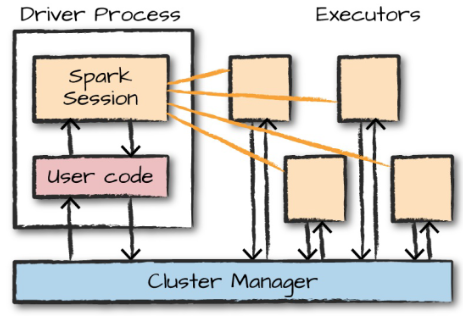
\includegraphics[height=5cm]{images/Screenshot_258.png}
	\end{center}
		\caption{Opbouw en structuur van een Spark-applicatie}
\end{figure}


\subsubsection{Partitionering}

Parallelle verwerking met Spark kan enkel gebeuren wanneer het systeem in verschillende clusters is opgebouwd. Een partitie is in dit geval een verzameling van rijen die op een fysieke machine in een cluster is opgeslaan. De partities van een DataFrame tonen hoe de data fysiek is verdeeld over de cluster heen. Het aantal partities is gebonden op het niveau van parallelisme in een Spark applicatie. Als je één partitie hebt, dan ga je een parallelisme van één hebben, zelfs al heb je meerdere executors. Omgekeerd ook, want als je meerdere partities hebt met één executor, dan zal je nog steeds een parallelisme van één hebben. De afweging maken tussen aantal partities en aantal executors speelt hier een rol op het vlak van snelheid.

\section{Spark in Java}

\subsection{Dataframe}

Een dataframe is een gedistribueerde, in-memory tabel met benoemde kolommen en een schema. Het schema duidt elke specifiek datatype aan. Een dataframe is \textit{immutable}, dus eenmaal aangemaakt kan het object niet meer worden gewijzigd. Dataframes kunnen worden aangemaakt uit verschillende bronnen, zoals Hadoop InputFormats of CSV-bestanden. Verdere transformaties, zoals aggregaties en filteren, kunnen zeker toegepast worden op eender welk type formaat. In Java-code verwijzen we naar het object 'Dataset<>'. Tussen de diamandtekens plaatsen we het object 'Row'.

\subsection{Transformaties}

Er zijn verschillende types transformaties die op een dataframe kunnen worden uitgevoerd. Deze transformaties verlopen \textit{lazy evaluated}. Het onderscheid tussen \textit{wide} en \textit{narrow} transformaties wordt hier gemaakt:

\begin{itemize}
	\item Een narrow transformatie is wanneer het resultaat voor een partitie kan worden berekend met enkel de data van die partitie. Iedere inputpartitie contribueert tot minstens één outputpartite. Deze transformatie kan ook gebeuren aan de hand van een pipeline, zo hoeft er geen data naar de disk te worden geschreven. Narrow transformaties zijn snel en efficiënt.
	\item Een wide transformatie heeft nood aan meerdere outputpartities. Sommige inputpartities zullen contribueren tot elk meerdere outputpartities. Hier is er nood aan een \textit{shuffle}, waarbij er een proces wordt toegevoegd. In dit proces worden de partities, over een cluster heen, onderling met elkaar uitgewisseld. Een shuffle vereist dat er resultaten naar de \textit{disk} wordt geschreven. Aangezien dit extra schrijfoperaties zijn, is het aangeraden om het aantal wide-transformaties zo minimaal mogelijk te houden.
\end{itemize}

\subsubsection{Lazy Evaluation}

Spark maakt gebruik van Lazy evaluation, wat wilt zeggen dat een transformatie niet zal resulteren in een nieuwe dataframe. De return-waarde is wél een nieuw object dat het resultaat van de bewerking bijhoudt. De berekening is nog niet uitgevoerd. Bij het triggeren van een actie kijkt Spark naar de graph van alle transformaties die werden opgeroepen. Net zoals bij SQL wordt er een \textit{query execution plan} aangemaakt. Dit proces noemt \textit{query optimization}. Spark kan mogelijks meerdere filters en filters gaan samensteken, of het kan andere soorten optimizatie gaan toepassen om zo min mogelijk data te moeten verwerken.

\subsection{Acties}

Transformaties in Spark bouwen een logische transformatieplan op. Die geeft aan hoe de inputdata moet worden getransformeerd om de gewenste output te krijgen. Het transformatieplan wordt niet uitgevoerd tot de actie wordt getriggerd. Een actie geeft Spark de instructie om een resultaat of verzameling van transformaties te berekenen. Sommige voorbeelden van acties zijn:

\begin{itemize}
	\item Sommige rijen van een dataframe tonen.
	\item Het aantal rijen van een dataframe optellen.
	\item De dataframe opslaan als een native object, zoals een Java lijst.
	\item Een dataframe schrijven naar een externe \textit{data sink}.
\end{itemize}

Eenmaal de actie is getriggerd, dan zal Spark het transformatieplan uitvoeren en de resultaat van de actie berekenen. 

\subsection{Physical plan}
Spark's Physical Plan wijst aan hoe de Spark-applicatie zal uitgevoerd worden op een cluster van machines. Dit omvat details zoals:
\begin{itemize}
	\item Welke transformaties moeten er worden uitgevoerd?
	\item Hoe moet de data gepartitioneerd of geshuffled worden?
	\item Hoe moeten de resultaten van de transformaties worden opgeslaan of geretourneerd?
\end{itemize}

\subsubsection{Het belang van een physical plan}

Het \textit{physical plan} is belangrijk, want zo achterhalen ontwikkelaars hoe zij hun middelengebruik kunnen optimaliseren en het aantal data, dat tussen machines heen moet worden geschreven, kan geminimaliseerd worden. Verdere oplossingen zijn:

\begin{itemize}
	\item Debugging en troubleshooten.
	\item Performance optimization
	\item Resource management
	\item Capaciteitsplanning
\end{itemize}

\section{Spark Libraries}

Dit is puur informatief. Spark bevat meerdere libraries om data-analyse of data-berekeningen op uit te voeren.

\begin{itemize}
	\item SQL en dataframe
	\item Spark Streaming
	\item MLLib
	\item GraphX
\end{itemize}

\subsection{Integratie met opslagsystemen}

Spark is ontworpen om met verschillende externe systemen te werken. Het is \textit{storage-system agnostic}, wat wilt zeggen dat het met een breed gamma aan storage systemen kan werken. Enkele voorbeelden van Spark-geïntegreerde storage systemen zijn:

\begin{itemize}
	\item HDFS is de populairste keuze voor Big Data, zowel gestructureerde als non-gestructureerde data.
	\item Key-value stores
	\item Relationele databanken
\end{itemize} 

\subsection{Resilient Distributed Dataset}

Voor Apache 2.0 werd er gewerkt met een Resilient Distributed Dataset of RDD object. Dit is een verzameling van objecten die parallel gemanipuleerd kunnen worden. Het is een fouttolerante werkwijze. RDD's zijn ook immutable en ze worden aangemaakt wanneer er wordt gelezen van een databron. RDD's zijn meer in de achtergrond verdwenen bij de nieuwere versies, maar ze blijven toegankelijk. RDD's komen in deze cursus niet meer aan bod.

\section{Spark-applicaties schrijven}

\subsection{Een dataframe met nieuwe waarden aanmaken.}

Stap voor stap wordt de volgende code uitgelegd:

\begin{enumerate}
	\item Eerst wordt er een spark-object aangemaakt in de main-methode. Zonder deze kan de applicatie niet werken.
	\item Er wordt een nieuwe lege lijst aangemaakt. We houden een Java-lijst bij van "Row's", ofwel de inhoud voor de dataframe.
	\item We maken vijf nieuwe rijen aan. In iedere rij houden we twee waarden bij: tekst en een getal. Met de RowFactory wordt er een Row-object aangemaakt, om dan vervolgens aan de Java-lijst toe te voegen.
	\item De komende twee stappen zijn optioneel, maar aan te raden. De ambitie is om een schema op te stellen. Het schema is een weergave van alle datatypes die in de dataframe aan bod komen. Zonder een schema moet Spark zelf uitvissen wat de datatypes zijn, en zelfs dan is er géén garantie dat het de juiste datatype is. In dit geval zijn er twee velden: naam in de vorm van een String en leeftijd in de vorm van een Integer. Deze lijst houdt de StructFields of schemavelden bij die in een schema moeten voorkomen. Dit is het schema nog niet!
	\item Op basis van de lijst met datatypes wordt er een schema gemaakt. Het schema is van het type StructType.
	\item Het dataframe wordt aangemaakt. Hiervoor komt het Spark-object van pas. Samen met de lijst van rijen als eerste parameter én het schema wordt het dataframe aangemaakt.
	\item Vervolgens wordt de data gegroepeerd op basis van naam. Zo zijn er twee Brooke's in het dataframe. In het resultaat zal er maar één Brooke te vinden zijn, maar van de twee leeftijden wordt het gemiddelde genomen.
	\item Het dataframe wordt in de terminal weergegeven. Alle kolommen, dus naam en leeftijd, worden weergegeven.
	\item Optioneel, maar wel aangeraden om het Spark-object te sluiten.
\end{enumerate}

\begin{lstlisting}[language=Java]
public	static void main(String[] args){
	
	SparkSession spark = SparkSession.builder()
									.appName("applicatiePersonenMetLeeftijd")
									.master("local[*]")
									.getOrCreate();
									
	List<Row> inMemory = new ArrayList<>();
	
	inMemory.add(RowFactory.create("Brooke",20));
	inMemory.add(RowFactory.create("Brooke",25));
	inMemory.add(RowFactory.create("Denny",31));
	inMemor.add(RowFactory.create("Jules",30));
	inMemory.add(RowFactory.create("TD",35));
	
	List<StructField> fields = Arrays.asList(
		DataTypes.createStructField("name",DataTypes.StringType, true),
		DataTypes.createStructField("age",DataTypes.IntegerType, true);
	)
	
	StructType schema = DataTypes.createStructType(fields);
	
	Dataset<Row> df = spark.createDataFrame(inMemory, schema);

	Dataset<Row> result = df.groupby("name").avg("age");
	
	result.show();
	
	spark.close();
}
\end{lstlisting}

\subsection{Een bestaande dataframe lezen}

Een dataframe wordt vaak gelezen uit een externe bron, zoals JSON, CSV, Parquet of Kafka output. Het Spark-object bezit een methode \textit{read()}. Deze methode geeft een DataFrameReader-object terug, wat nodig is om een bron in te lezen. Veronderstel dat we hier met dezelfde dataset te maken hebben, maar enkel al vooraf opgeslaan in een csv-bestand.

\begin{enumerate}
	\item Spark-object aanmaken.
	\item Schema maken door een lijst van StructFields te maken én die dan te gieten in een StructType-object.
	\item Het CSV-bestand wordt ingelezen. Net zoals het aanmaken, gebeurt het inlezen ook met het Spark-object. In het CSV-bestand is er een header, vandaar dat er eerst de optie 'header:true' wordt meegeven. Vervolgens wordt het schema meegegeven én uiteindelijk het pad waar de CSV kan worden teruggevonden.
	\item Net zoals daarnet wordt er gegroepeerd op naam. Per naam wordt de gemiddelde leeftijd teruggegeven.
	\item Het dataframe wordt in de terminal getoond.
\end{enumerate}

\begin{lstlisting}[language=Java]
public static void main(String[] args){
	
	SparkSession spark = SparkSession.builder()
								.appName("applicatiePersonenMetLeeftijd")
								.master("local[*]")
								.getOrCreate();
								
	List<StructField> fields = Arrays.asList(
			DataTypes.createStructField("name",DataTypes.StringType, true),
			DataTypes.createStructField("age",DataTypes.IntegerType, true);
	)
	
	StructType schema = DataTypes.createStructType(fields);
	
	Dataset<Row> df = spark.read()
						.option("header", true)
						.schema(schema)
						.csv("src/main/resources/PersonenMetLeeftijd.csv");
	
	Dataset<Row> result = df.groupby("name").avg("age");
	
	result.show();
	
	spark.close();
}
\end{lstlisting}

\subsubsection{Schema overerven}

In de vorige twee berekeningen werd er een schema zelf, door de ontwikkelaar, aangemaakt. Dit is vrijblijvend, want Spark kan ook een schema overerven. Hieronder is er een alternatieve methode op stap twee van het vorige voorbeeld. Deze methode is minder efficiënt, want Spark moet zelf achterhalen wat de meest geschikte datatypes zijn. Daarnaast gaat Spark lijn per lijn door de volledige dataset heen. Wel kan je de workload minimaliseren door het schema op te bouwen o.b.v. een deel van de volledige dataset. Dit is een deelse oplossing, want er kunnen nog steeds problemen voorkomen bij de gekozen datatypes. Daarom is het aangeraden om zelf een schema op te bouwen.

\begin{lstlisting}[language=Java]
Dataset<Row> df  = spark.read()
						.option("header", true)
						.option("inferSchema", true)
						.option("samplingRation", 0.0001)
						.csv("src/main/resources/PersonenMetLeeftijd.csv)
\end{lstlisting}

\subsection{Een dataframe uitschrijven naar een nieuw bestand.}

In de volgende code wordt er verondersteld dat er een Spark-object is aangemaakt, een schema is opgesteld én een dataset al is ingelezen. De dataset werd opgeslaan als DataFrame onder de naam 'result'.

\begin{enumerate}
	\item Het pad wordt tweemaal gebruikt, dus dat wordt opgeslaan onder een variabele. Het pad kan zowel relatief als absoluut zijn. In dit voorbeeld is het pad absoluut.
	\item Er zijn drie opties:
	\begin{enumerate}
		\item De inhoud van de dataframe wordt uitgeschreven naar een parquet-bestand. Dit bestand is een must bij een column-oriented databankstructuur.
		\item Vervolgens wordt de mode meegegeven. Bij het uitschrijven wordt er een map gegenereerd. In die map kan het parquet-bestand worden teruggevonden.
		\item Als laatste moet er een outputpad worden meegegeven. 
	\end{enumerate}
	\item Puur uit controle wordt het net aangemaakte bestand ingelezen door Spark. De outputpad, waar het parquet-bestand werd opgeslaan, dient nu als inputpad.
	\item Het Spark-object wordt gesloten.
\end{enumerate}

\begin{lstlisting}[language=Java]
String path = "file:///C:/tmp/personen";

df.write()
	.format("parquet")
	.mode("overwrite")
	.save(path);
	
Dataset<Row> dfParquet = spark.read().parquet(path);

spark.close();
\end{lstlisting}

\section{Dataframe-kolommen inlezen, toevoegen en verwijderen.}

\subsubsection{Kolommen toevoegen}
Een dataframe bestaat uit kolommen. Sommige functies vragen de naam van een kolom op als String, maar andere functies vereisen dat je een object van de klasse 'Column' meegeeft. In het volgende voorbeeld wordt er een extra kolom aangemaakt. De kolom is een berekening op de leeftijdskolom. 

\begin{enumerate}
	\item Bovenaan komen de imports. De klasse 'functions' is met een kleine letter geschreven, daarmee een uitzondering op de regel om alle klassen met een hoofdletter te laten starten.
	\item Er worden twee kolommen aan de dataset toegevoegd. Een expressie of where-clausule wordt meegegeven met de \textit{expr(...)}-functie.
\end{enumerate}

\begin{lstlisting}[language=Java]
import org.apache.spark.sql.Column;
import static org.apache.spark.sql.functions.col;

df = df.withColumn("ageNextYear2", expr("age + 1"))
			.withColumn("over30", expr("age > 30"));
\end{lstlisting}

\subsubsection{Kolommen selecteren}
Tot nu toe werden alle kolommen van de dataframes bij de keuze betrokken. Spark laat de ontwikkelaar toe om kolommen, net zoals bij SQL, te kiezen. Hieronder wordt er een voorbeeld gegeven van de verschillende kolommen. Er wordt verondersteld dat er al een spark-object is aangemaakt én dat het pad in een String 'inputpath' wordt bijgehouden.

\begin{enumerate}
	\item Er wordt een nieuwe dataset opgehaald. De dataset is opgeslaan in een CSV-bestand. Het bevat vijf kolommen: id, score, naam, jaartal en kwartaal. Enkel bij dit voorbeeld wordt het schema overgeërfd. 
	\item De dataset wordt in de terminal getoond. Alle vijf kolommen worden weergegeven.
	\item Met de \textit{select}-functie worden enkel de score, jaartal en kwartaalkolommen opgehaald. Een dataframe is \textit{immutable}, dus het object moet worden overschreven.
	\item De dataset bestaat nu uit drie kolommen. 'Id' en 'naam' zijn niet meer terug te vinden in de dataset.
\end{enumerate}

\begin{lstlisting}[language=Java]
Dataset<Row> df = spark.read()
						.option("header",true)
						.option("inferSchema",true)
						.option("sampleRation", 0.001)
						.csv(inputpath);

df.show();

df = df.select("score","jaartal","kwartaal");

df.show();
\end{lstlisting}

\subsubsection{Kolommen verwijderen}

Een kolom kan op een passieve wijze worden weggelaten door de kolom niet in een \textit{select} te betrekken. In sommige gevallen, bijvoorbeeld bij een groot aantal kolommen, is het handiger om één specifieke kolom te verwijderen, in plaats van een select uit te voeren. De gouden regel is dat dataframes immutable zijn, dus hier moet de nieuwe versie van de dataframe opnieuw wordt toegekend.

\begin{lstlisting}
df = df.drop("id","naam");
\end{lstlisting}

\subsubsection{Kolommen hernoemen}

Kolomnamen kunnen worden aangepast. Bij het toevoegen wordt er vaak een standaardnaam toegekend aan een kolom, bijvoorbeeld \textit{count} of \textit{sum}. Hieronder wordt de kolom met de naam \textit{count} aangepast naar \textit{aantalRijen}. Na een berekening kan je ook de \textit{alias}-functie gebruiken. 

\begin{lstlisting}[language=Java]
df = df.withColumnRenamed("count","aantalRijen");
df = df.count().alias("aantalRijen");
\end{lstlisting}

\subsection{Dataframes filteren}

\subsubsection{Voorbeelden van de studentendataset}

\begin{enumerate}
	\item Hou een dataset bij met alle rijen die een score hebben van 'A+'.
	\item Hou een dataset bij met alle rijen waarvan de score 'B' is én de score werd behaald in het jaar 2010 of 2011.
	\item Neem de dataset van nummer 3 en behoud enkel de unieke rijen.
\end{enumerate}

\begin{lstlisting}[language=Java]
Dataset<Row> dfAplus = df.select()
						.where(col("grade")
						.equalTo("A+");
						
Dataset<Row> dfB1011 = df.select()
						.where(col("grade").equalTo("B")
										.and(col("year").isin(2010,2011)));
						
Dataset<Row> dfUniekB1011 = dfB1011.distinct();
\end{lstlisting}

\subsection{Aggregaties uitvoeren op dataframes}

\subsubsection{Voorbeelden van de studenten-dataset}

\begin{lstlisting}[language=Java]
Dataset<Row> dfCountPerJaar = df.select("year")
			.groupby("year")
			.count()
			.orderBy(desc("count"));
			
Dataset<Row> dfStatisticsPerJaarEnOnderwerp = df.select("year","subject","score")
			.groupby("year","subject")
			.agg(max("score"), min("score"), avg("score"))
			
\end{lstlisting}

\subsubsection{Voorbeelden van de ViewingFigures-oefening}

\begin{lstlisting}[language=Java]
Dataset<Row> chaptersPerCourse = chaptersDF
									.drop("chapterId")
									.groupBy("courseId").count()
									.withColumnRenamed("count", "chapters");
\end{lstlisting}


\subsection{User Defined Functions}

User Defined Functions of UDF's worden ingezet wanneer een berekening de ingebouwde functies van Spark overstijgt. De berekening maken is mogelijk, maar de logica is te complex en vereist daarmee een aparte aanpak. Bij een UDF zijn er drie stappen:

\begin{enumerate}
	\item UDF schrijven.
	\item UDF registreren.
	\item UDF oproepen.
\end{enumerate}

\begin{lstlisting}[language=Java]
UDF1<Double, Integer> score = new UDF1<Double, Integer>() {
	public Integer call(Double percent) throws Exception {
		if (percent > 0.9) {
			return 10;
		} else if (percent > 0.5) {
			return 6;
		} else if (percent > 0.25) {
			return 2;
		} else {
			return 0;
		}
	}
};

spark.udf().register("berekenScore", score, DataTypes.IntegerType);


Dataset<Row> result = percentageDF
	.withColumn("score",  call_udf("berekenScore",col("percentage")))
	.drop("percentage")
	.groupBy("courseId").agg(sum("score").as("total"))
	.join(titleDF, "courseId")
	.orderBy(desc("total"));
\end{lstlisting}

\chapter{Spark Streaming}

Batch processing: 
* Wanneer de winkel dichtgaat --> verslag van alles wat verkocht werd die dag = data in een batch
* Moeilijk wanneer je iets real-time wilt doen. De status van de data is belangrijk.

\subsection{Spark Structured Streaming}

'Data is unbounded'.

* Nieuwe rijen worden continu achteraan toegevoegd.
* Probleem: We houden geen oneindige tabel in het geheugen. 
* ...

Gelijkaardig aan een SQL API:
* Unbounded table, maar het systeem denkt niet zo.
* Eén API nodig om zowel batch als stream processing uit te voeren.
* Je schrijft je query zoals je batch processing hebt.
* Job triggeren om data te verkrijgen. Iedere keer als de job start, Spark zal kijken voor nieuwe data.

### Output modes

Append mode:
* Enkel nieuwe rijen toevoegen (resultaat)
* Historiek / bestaande rijen worden niet getoond of aangepast.
* Standaard
* Niet mogelijk bij WordCount: het aantal voorkomens wordt niet lang bijgehouden.

Update mode:
* Nieuwe rijen \& oude rijen.
* Sommige "sinks" ondersteunen dit niet. Alles waar je de rijen naar toe schrijft.
* Bestanden hebben geen interne structuur, eenmaal een bestand geschreven is dan is het moeilijk om dit aan te passen. Bijvoorbeeld als de vorige rij 5 kolommen heeft en nu komt er een rij met 6 ==> error.

Complete:
* Het volledige resultaat wordt uitgeschreven
* De output zal stelselmatig groeien. De job zal niet draaien
* Gebruiken bij aggregation.

Bij een socket lees je enkel hetgeen wat binnenkomt. Historiek wordt niet bijgehouden.

\section{Code}

Er zijn vijf stappen:

\section{Input source}

readStream om een stream van objecten in te lezen
* format: sockets, etc.
* options: Kafka --> wie is de broker
* load: dit is het beginnen met lezen, niet wanneer alles wordt gelezen.

\begin{lstlisting}[language=Java]
Dataset<Row> df = spark.readStream()
	.format("socket")             // lezen van een socket
	.option("host", "localhost")  // optie: host
	.option("port", 9999)         // optie: poortnummer
	.load();
\end{lstlisting}

```

\subsection{Transform data}

Je hebt enkel de huidige data nodig.

Stateful \& stateless:
* Loopt parallel met "wide \& narrow"
* stateful: de huidige informatie is voldoende (bijvoorbeeld mapping)
* stateless: je hebt informatie van voordien nodig (bijvoorbeeld een groupby of een aggregatie)

\subsection{Output}

* Geef mee waarnaartoe je de data wilt schrijven.
* outputMode

\begin{lstlisting}
Dataset<Row> counts = ....
DataStreamWriter<Row> writer = counts.writeStream()
	.format("console")
	.outputMode(OutputMode.Complete());
\end{lstlisting}

\subsection{Processing Details}

Micro-batches heel snel uitvoeren. Je moet meegeven wanneer de volgende micro-batch wordt uitgevoerd. 
* Standaard: zo snel na de laatste micro-batch alles verwerken.
* Trigger interval: gelijkaardig aan Cronjobs. Op een bepaald moment wordt de query uitgevoerd.
* Eenmalig: "Verwerk alle data nu en stop dan."
* Continuous: De data wordt niet in micro-batches verwerkt. Zo snel als het binnen komt wordt de data verwerkt. Hier is er weinig vertraging. Dit is eerder voor een experimenteel gebruik.

\begin{lstlisting}
DataStreamWriter<Row> writer = counts.writeStream()
	.format("console")
	.outputMode(OutputMode.Complete())
	.trigger(Trigger.ProcessingTime(1,TimeUnit.SECONDS));
\end{lstlisting}


\subsection{Query starten}

\begin{lstlisting}
StreamingQuery streamingQuery = writer.start();
try{
	
	} except {
	
};
\end{lstlisting}

\subsection{Sources \& Sinks}

Uit bestanden of directories lezen:

* Parallel applicaties uitvoeren.
* Geen garantie welk bestand er eerst wordt bekeken.
* Naar een bestand schrijven --> enkel append mode mogelijk

Uit Kafka lezen:

* Het schema bij Kafka Dataframees zal altijd hetzelfde zijn. De key-value wordt als binary teruggegeven, maar dit is in binary. Parsen is noodzakelijk.

Naar Kafka schrijven:

* Kolomnamen staan vast. 
* Schrijven van topic naar topic(s) is mogelijk.

\subsection{Map to overlapping windows}

Iedere timestamp wordt naar een windows gemapt.
* groupby op interval en word
* truncate op false: altijd volledige woord


Watermark delay:
* keeps state bounded


Event time (ET): 
* moment wanneer iets aangemaakt werd bij de bron
* de watermark gaat kijken naar de grootste event time.

Watermark:
* "Bezemwagen": telkens de laatste timestamp updaten.
* Ieder ET met een ET voor 12u10: wordt niet meegeteld.
* [12u - 12u10]
* State wordt telkens kleiner.
* 

```java
.withWatermark()
```

\subsection{Join streams}

Static DF + Stream:
* Left Outer, Inner of Right Outer.
* Enkel Outer met de streaming

Geen watermarking nodig:
* Stream met een bounded-ding: geen state van de DF nodig.

Caching:
* Iedere n aantal seconden een DF lezen: alles cachen.
* Static DF

```java
.cache()
```

\subsection{Stream-Stream joins}


\chapter{Kafka}

Check out Learn Apache Kafka for Beginners.

\section{Transporting data}

Source: Maakt data.
Target: Verbruikt data.

| w/ | wo/ |
| -- | -- |
|  Kafka functioneert hier als tussenpersoon. De tussenpersoon zal het verkeer naar de targets regelen. Zo moeten de sources niet verbonden zijn met alle targets. Dit zorgt voor een fouttolerant en veerkrachtig systeem. Kafka staat ook sterk bij horizontale schaalbaarheid. | Iedere source is verbonden met ieder target. Dit is de meest verbruikende manier van de twee. Hier moet iedere source rekening houden met protocollen, doorvoer, etc. |
| m + n | m x n|


\section{Topics}
Topics:
* Stream van data. Meerdere mogelijk.
* Naamgeving.
* Wordt opgedeeld in een **vast aantal partities**:

\section{Partitions}
* Doorvoer verbeteren
* Een bestand op een lokaal FS.
* Append-only. Je kan enkel messages op het einde toevoegen.
* Offset = 0 : Allereerste bericht. 
* Offset van de laatste partitie = n
* Bij vergissing: pech!
*  Je kan het niet verwijderen of aanpassen.
*  Een dubbele actie (bv.: twee messages rond een aankoop): Je moet een derde message sturen om de dubbel ongedaan te maken.
* Ordening is niet gesorteerd!
* min -> max
* Je kan het aanpassen (?), maar er hangen hier nadelen aan.


\section{Kenmerken}
* Immutable
* Limited: Volgens de default policy worden berichten ouder dan een week verwijderd.
* Je specifieert de topic waar het bericht naartoe moet, niet de partition.
* Partitie is willekeurig --> Load-balancing

\section{Rollen}

\subsection{Broker}
= Computer

* Elke broker een ID geven.
* Elk bestaat uit partities 
* --> weinig controle over de brokers: geen master/slave verhouding.
* Als je één broker kent, dan kan je verbinding maken met alles binnen de cluster.
* Per standaard: drie brokers.
* één broker ook mogelijk: geen schaalbaarheid.

Partitie toekennen aan broker(s):
* Algoritme

\subsection{Leader}

Leader/followers:
* Leaders hebben volledige toegang tot de data.
* Moet worden aangesproken als er iets in de partitie moet worden veranderd

\subsection{Follower}

Volgers hebben geen toegang. 
* Gedrag kan worden beïnvloed.
* Een applicatie binnen dezelfde rack als een follower, van de data dat die nodig heeft, zal de volger aanspreken i.p.v. leader.


\section{Data Replication}
Het repliceren van data:
* Fouttolerantie: voorkomen dat data verloren raakt als het systeem van een partitie defunct gaat.
* Partitioneren verhoogt de schade bij een fout.

Replication factor:
* Factor hoger dan één, maar niet te hoog!
* Broker kapot --> andere broker bezit de data

**Out-of-sync**: De volger beschikt niet meer over de meeste recente data.

**Fetch requests**: Geef mij alles dat begint vanaf deze offset.
* De replica weet hoeveel offsets die achterloopt op de leider.
* **In-sync**: er is geen verschil tussen de replica en de leider. Enkel zij komen in aanmerking om leider te worden.
* Als de leider geen fetch request ziet voor meer dan 10 seconden == Out-of-Sync (Mortis)

\subsection{Producer}
* Schrijft/verstuurt data naar de topic(s).
* Zal automatisch opnieuw proberen.

| Hoe achterhalen of een bericht is toegekomen: | -- | |
| -- | -- | -- |
| Bericht versturen + schietgebedje | ack=0 | Unreliable, maar snel. |
| Bericht versturen + wachten op bevestiging | acks=1 | Deels geruststellend. |
| Bericht versturen en wachten tot de leider + in-sync replicas het bericht hebben ontvangen. | acks=all | Volledige geruststelling, maar gevaarlijk als er géén enkele replica in-sync is. Geen in-sync replicas: enkel de leader wordt geüpdatet. Als er géén in-sync replica's zijn is alles *'goed'* verlopen. Dit voorkom je door *min in-sync replica's* op twee te plaatsen. Nooit hetzelfde getal als je replication factor (vb.: 2 & 2), want dan verwacht je dat je geen trage volgers hebt. |

\subsection{Consumer}
* Data lezen van de topic(s)
* Toekennen aan partitie:
* Speciale topic binnen Kafka: Consumer offset.


Consumer offset:
* De staat van topics.
* Logboek: "ik heb de messages t.e.m. 50 gelezen". 
* Achterhalen vanaf waar de consumer berichten moet verwerken.

## Delivery Semantics
* "Wat kan een consumer doen om het bericht te verwerken?"
* "Wanneer vertel je Kafka dat je klaar bent met het verwerken van een bericht?"


## Zookeeper
* leader-follower architecture


\section{Labo}

We moeten hier het poortnummer 19092 gebruiken voor Kafka1. 

```cmd
kafka-topics --bootstrap-server kafka1:19092 --list
kafka-topics --bootstrap-server kafka2:19093 --list
kafka-topics --bootstrap-server kafka3:19094 --list
```

Het maakt niet uit bij welke broker. De actie zal altijd werken.

Aanmaken:
```cmd
kafka-topics --create --topic lecture --partitions 3 --replication-factor 3
```

Omschrijven:
```cmd
kafka-topics --bootstrap-server kafka1:19092 --describe --topic lecture
```

Nieuwe messages toevoegen:
```cmd
kafka-console-producer --bootstrap-server kafka1:19092 --topic-lecture
```
	
\end{document}